%% LyX 1.5.5 created this file.  For more info, see http://www.lyx.org/.
%% Do not edit unless you really know what you are doing.
\documentclass[a4paper,czech,czech,openright,cleardoubleempty,BCOR10mm,DIV11]{scrreprt}
\usepackage[T1]{fontenc}
\usepackage[utf8]{inputenc}
\usepackage{array}
\usepackage{longtable}
\usepackage{varioref}
\usepackage{wrapfig}
\usepackage{fancybox}
\usepackage{calc}
\usepackage{framed}
\usepackage{url}
\usepackage{graphicx}
\usepackage{color}
\usepackage{float}
\usepackage{svg}
\usepackage{amsmath}
\usepackage{makecell}
\usepackage{fourier} 
\usepackage{pdfpages}

\makeatletter

%%%%%%%%%%%%%%%%%%%%%%%%%%%%%% LyX specific LaTeX coěmmands.
\providecommand{\LyX}{L\kern-.1667em\lower.25em\hbox{Y}\kern-.125emX\@}
\newcommand{\lyxline}[1][1pt]{%
  \par\noindent%
  \rule[.5ex]{\linewidth}{#1}\par}
\newcommand{\noun}[1]{\textsc{#1}}
%% Special footnote code from the package 'stblftnt.sty'
%% Author: Robin Fairbairns -- Last revised Dec 13 1996
\let\SF@@footnote\footnote
\def\footnote{\ifx\protect\@typeset@protect
    \expandafter\SF@@footnote
  \else
    \expandafter\SF@gobble@opt
  \fi
}

\expandafter\def\csname SF@gobble@opt \endcsname{\@ifnextchar[%]
  \SF@gobble@twobracket
  \@gobble
}
\edef\SF@gobble@opt{\noexpand\protect
  \expandafter\noexpand\csname SF@gobble@opt \endcsname}
\def\SF@gobble@twobracket[#1]#2{}
%% Because html converters don't know tabularnewline
\providecommand{\tabularnewline}{\\}

%%%%%%%%%%%%%%%%%%%%%%%%%%%%%% Textclass specific LaTeX commands.
\newenvironment{lyxcode}
{\begin{list}{}{
\setlength{\rightmargin}{\leftmargin}
\setlength{\listparindent}{0pt}% needed for AMS classes
\raggedright
\setlength{\itemsep}{0pt}
\setlength{\parsep}{0pt}
\normalfont\ttfamily}%
 \item[]}
{\end{list}}

%%%%%%%%%%%%%%%%%%%%%%%%%%%%%% User specified LaTeX commands.
%<-------------------------------společná nastavení------------------------------>
\usepackage[czech]{babel}%počeštění názvů (Obsah, Kapitola, Literatura atp.)
\usepackage[]{hyperref} %odkazy v  pdf jsou klikací s barevnými rámečky
\usepackage[numbers,sort&compress]{natbib} %balíček pro citace literatury  
\usepackage{hypernat}%interakce mezi hyperref a natbib
\newcommand{\BibTeX}{{\sc Bib}\TeX}%BibTeX logo
\hypersetup{   % Nastavení polí PDF dokumentu 
pdftitle={Evaluation of Container-based Virtualization for standard company environment},%   
pdfauthor={Pavel Cizinsky},%  
pdfsubject={},%   
pdfkeywords={Docker, Kubernetes, Kotejner, Virtualizace}%                             
}
\usepackage{multicol}




%<-----------------------------volání stylů----------------------------------------->
% (znak % je označení komentáře: co je za ním, není aktivní)
%<------------------------------------písmo----------------------------------------->
%\usepackage{packages/bc-latinmodern}
%\usepackage{packages/bc-times}
\usepackage{packages/bc-palatino}
%\usepackage{packages/bc-iwona}
%\usepackage{packages/bc-helvetika}


%<------------------------------záhlaví stránek------------------------------------>
%\usepackage{packages/bc-headings}
\usepackage{packages/bc-fancyhdr}

%<------------------------------hlavičky kapitol------------------------------------>
%\usepackage{packages/bc-neueskapitel}
%\usepackage{packages/bc-fancychap}

\makeatother

\usepackage{babel}

%java code block%

\usepackage{listings}
\usepackage{color}

\definecolor{dkgreen}{rgb}{0,0.6,0}
\definecolor{gray}{rgb}{0.5,0.5,0.5}
\definecolor{mauve}{rgb}{0.58,0,0.82}

% syntax highlight pro jazyk Javascript %
\definecolor{purple}{rgb}{0.65, 0.12, 0.82}
\lstdefinelanguage{JavaScript}{
  keywords={break, case, catch, const, continue, debugger, default, delete, do, else, false, finally, for, function, if, in, instanceof, let, new, null, return, switch, static, this, throw, true, try, typeof, var, void, while, with},
  morecomment=[l]{//},
  morecomment=[s]{/*}{*/},
  morestring=[b]',
  morestring=[b]",
  ndkeywords={class, constructor, export, extends, boolean, throw, implements, import},
  keywordstyle=\color{blue}\bfseries,
  ndkeywordstyle=\color{gray}\bfseries,
  identifierstyle=\color{black},
  commentstyle=\color{purple}\ttfamily,
  stringstyle=\color{red}\ttfamily,
  sensitive=true
}

\lstset{,
  language=Javascript,
  aboveskip=3mm,
  belowskip=3mm,
  showstringspaces=false,
  columns=flexible,
  inputencoding=utf8,
    extendedchars=true,
    literate=%
    {á}{{\'a}}1
    {č}{{\v{c}}}1
    {ď}{{\v{d}}}1
    {é}{{\'e}}1
    {ě}{{\v{e}}}1
    {í}{{\'i}}1
    {ň}{{\v{n}}}1
    {ó}{{\'o}}1
    {ř}{{\v{r}}}1
    {š}{{\v{s}}}1
    {ť}{{\v{t}}}1
    {ú}{{\'u}}1
    {ů}{{\r{u}}}1
    {ý}{{\'y}}1
    {ž}{{\v{z}}}1
    {Á}{{\'A}}1
    {Č}{{\v{C}}}1
    {Ď}{{\v{D}}}1
    {É}{{\'E}}1
    {Ě}{{\v{E}}}1
    {Í}{{\'I}}1
    {Ň}{{\v{N}}}1
    {Ó}{{\'O}}1
    {Ř}{{\v{R}}}1
    {Š}{{\v{S}}}1
    {Ť}{{\v{T}}}1
    {Ú}{{\'U}}1
    {Ů}{{\r{U}}}1
    {Ý}{{\'Y}}1
    {Ž}{{\v{Z}}}1,
  basicstyle={\small\ttfamily},
  xleftmargin=1cm,
  keywordstyle=\color{blue},
  commentstyle=\color{dkgreen},
  stringstyle=\color{mauve},
  breaklines=true,
  breakatwhitespace=true,
  tabsize=3
}
\usepackage{url}
\makeatletter
\g@addto@macro{\UrlBreaks}{\UrlOrds}
\makeatother

% vlastni package
\usepackage{placeins}
\usepackage{multirow}
\usepackage{pdfpages}
% fonty popisku
\usepackage[font=small,labelfont=bf]{caption}
% radkovani 
\renewcommand{\baselinestretch}{1.2}
\renewcommand*{\lstlistingname}{Kód} %prejmenovani lstlisting
\renewcommand*{\lstlistlistingname}{Seznam ukázek kódu}
% vlastni styly tabulek
\newcolumntype{C}[1]{>{\centering\arraybackslash}m{#1}}
\begin{document}

\cleardoublepage{}~\thispagestyle{empty}\begin{center}\pagenumbering{roman}\vspace{10mm}


\textsf{\textsc{\noun{\LARGE Univerzita Hradec Králové}}}\\
\vspace{0.5em}
\textsc{\noun{\LARGE Fakulta informatiky a managementu}}\\
\vspace*{1em}
\textsf{\textsc{\noun{\Large katedra informačních technologií }}}


%%% Aby vložení loga  správně fungovalo, je třeba mít soubor uhk.png nahraný v adresáři logo,
%%% tj. v adresáři, kde se nachází překládaný zdrojový soubor. 
\vspace{4cm}

\textsf{\huge BAKALÁŘSKÁ PRÁCE}{\huge \par}

\vspace{15mm}


\textsf{\LARGE Využití kontejnerové virtualizace pro standardní firemní prostředí}{\LARGE \par}

\vspace{10mm}


\end{center} 

\vspace*{\fill}


\vspace{10mm}


\begin{description}
%studijni obor???
\item [{{\large Autor:}}] \noindent \textsf{\large Pavel Čižinský}{\large \par}
\item [{{\large Studijní obor:}}] \noindent \textsf{\large Aplikovaná informatika}{\large \par}
\item [{{\large Vedoucí~práce:}}] \noindent \textsf{\large Ing. Jakub Pavlík, MSc.}{\large \hfill{}}\textsf{\large Hradec Králové, 2017}{\large{}
% doplňte rok vzniku vaší bakalářské práce
}{\large \par}
\end{description}

\clearpage{}
~\thispagestyle{empty}{\small ~\vfill{}
}{\small \par}

\noindent {\small \vfill{}
 % nastavuje dynamické umístění následujícího textu do spodní části stránky
~}{\small \par}

\noindent {\small Prohlašuji, že jsem bakalářskou práci vypracoval samostatně a uvedl jsem všechny použité prameny a literaturu.}{\small \par}

{\small \bigskip{}
}\noindent {\small{} V Jaroměři dne \today\hspace{\fill}Pavel Čižinský}\\
{\small{} % doplňte patřičné datum, jméno a příjmení
}{\small \par}

{\small %%%   Výtisk pak na tomto míste nezapomeňte PODEPSAT!
%%%                                         *********
}{\small \par}

\clearpage{}
~\thispagestyle{empty}{\small ~\vfill{}
}{\small \par}

\noindent {\small Rád bych poděkoval Ing. Jakubu Pavlíkovi, MSc. za odborné vedení práce, podnětné rady a čas, který mi věnoval. \newpage{}}{\small \par}
\clearpage{}
~\thispagestyle{empty}{\small ~\vfill{}
}{\small \par}
\noindent {\small \vfill{}
 % nastavuje dynamické umístění následujícího textu do spodní části stránky
~}{\small \par}
\section*{Anotace}
Tato bakalářská práce pojednává o kontejnerové virtualizaci, zabývá se problematikou nasazení kontejnerů do standardního firemního prostředí. První část je věnována představení virtualizace obecně a její porovnání s kontejnerovou virtualizací. Následně je řešena problematika orchestrace a ovládání kontejnerového prostředí. Čtvrtá a pátá kapitola je věnována analýze a převodu aplikace do kontejnerů, součástí  kapitoly pět je praktická ukázka funkčnosti orchestrátoru. Cílem této práce je seznámení čtenáře s konceptem kontejnerů a zjistit jejich využitelnost v produkčním prostředí a možnost převodu klasické aplikace do kontejnerů.
\subsubsection*{Klíčová slova}
Docker, Kubernetes, Cluster, Kontejnery, Virtualizace

\section*{Annotation}
Title: Evaluation of Container-based Virtualization for standard company environment
\vspace{0.5cm}\FloatBarrier
This Bachelor’s thesis describes container-based virtualization especially the issues in its use in standard company environment. The first part is dedicated to intruducing general virtualization and its comparison to container-based virtualization. Afterward is tackled the troubleshooting of orchestration and control of the container-based environment.
The fourth and fifth chapters are devoted to the analysis and conversion of application into containers. Practical example of the orchestration's functionality is included in chapter five.
The aim of this work is to familiarize the reader with the concept of containers and to find out their applicability in the production environment as well as the ability to convert a classic application into containers.

\subsubsection*{Key words}
Docker, Kubernetes, Cluster, Containers, Virtualization

\noindent {\small ~\vfill{}
}{\small \par}

\cleardoublepage{}\thispagestyle{empty}{\small \tableofcontents{}% vkládá automaticky generovaný obsah dokumentu
\cleardoublepage{}}{\small \par}

\chapter{Úvod}
\pagenumbering{arabic}
\setcounter{page}{1}
Kontejnery pro virtualizaci existují již řadu let. Rozšíření kontejnerů přišlo před čtyřmi lety s firmou Docker a jejich technologiemi. Hlavní rozdíly mezi kontejnery a klasickou virtualizací jsou ve spotřebě zdrojů. \newline
Pro virtualizaci založenou na kontejnerech je klíčové sdílení systémových zdrojů s hostitelským operačním systémem, oproti klasické, která celý systém ve virtuálním stroji emuluje a vytváří tak vlastní zdroje.

Práce s dnešními kontejnerizačními nástroji je velmi jednoduchá a intuitivní. Během krátké doby začaly používat kontejnerové technologie ve svých infrastrukturách firmy jako Spotify, Yahoo či Google\cite{docker_part}. Můžeme předpokládat, že s rozšiřováním cloudových služeb se bude také zvyšovat zapojování kontejnerů.

V dnešní době rychlého škálování a růstu firem je velmi důležitá dynamika, pomocí které je možné kontejnery spravovat.

Práce je zaměřená na prozkoumání problematiky kontejnerové virtualizace. Cílem práce je převedení aplikace a zjištění, jaký orchestrátor je pro produkční kontejnerové prostředí optimální.

Obsah bakalářské práce je rozčleněn do 6 kapitol. V následující kapitole je popsán princip kontejnerů a porovnání kontejnerových technologií. V kapitole 3 je vysvětlen princip orchestrátoru a porovnání jednotlivých typů. Kapitola 4 se zaměřuje na analýzu migrované aplikace a výběr vhodných nástrojů pro migraci. Migrace této aplikace je pak  popsaná v kapitole 5. Závěrečná kapitola 6 je věnována shrnutí výsledků praktické práce a doporučením.

V bakalářské práci se vyskytují anglické výrazy. Výrazy, které nemají české ekvivalenty, nebudou v této práci přeloženy tak,u jak je v technických publikacích běžné.

\chapter{Principy kontejnerové virtualizace} \label{chp:kontejner}
První bod této kapitoly se zabývá obecnou historií kontejnerů. K vyjasnění principů pro kontejnerovou virtualizaci je třeba vysvětlit dva základní pojmy, virtualizaci a kontejner.

\section{Historie kontejnerové virtualizace}
První pokusy o kontejnerizaci pocházejí už z roku 1979, kdy bylo možné pro izolaci aplikací a procesů využít chroot. Tento koncept je ovšem velmi jednoduchý a má svá omezení.
V roce 2000 byl chroot zdokonalen v rámci projektu FREEBSD jails\cite{chroot}, taktéž znám pod jménem Chroot on Steriods\cite{chroot}. Toto řešení již bylo pokročilejší, dokázalo plně izolovat proces, byla zde vyřešena podpora pro networking. Vzhledem k malému rozšíření systému FREEBSD se tento projekt dlouhodobě nepoužíval.

Se svým konceptem kontejnerů se představil také Oracle. Projekt se nazýval solaris zones\cite{solaris_zone} (Solaris Containers). Řešení bylo velmi podobné existujícím kontejnerům s lépe vyřešenými požadavky na file systém a podporou ZFS.
V roce 2005 se začala firma Google potýkat s problémy, jak přenášet své webové služby. Google již nějakou  dobu experimentoval s kontejnery pro tuto potřebu, ale zjistil, že se jedná o nevhodné řešení. Hlavní problém byl výkon, který byl příliš slabý a odezva příliš pomalá na to, aby kontejnery dokázaly pracovat s požadovanými webovými službami.

Ve stejném období začali budoucí pracovníci Googlu experimentovat s linuxovým konceptem postaveným na cgroups (control groups), nazývaným jako procesové kontejnery. Za několik měsíců stejná skupina inženýrů pomocí těchto kontejnerů vyřešila problém se škálovatelností jednotlivých data center Googlu. 
V lednu 2008 byly některé cgroup technologie, které používal Google, přidané do Linuxového jádra, čímž daly základ projektu LXC (LinuX Containers).

V roce 2013 společnosti Google a Parallels odsouhlasily spolupráci. Výsledkem bylo vydání Linuxového jádra ve verzi 3.8\cite{gp_38}, které obsahovalo jejich linuxové virtualizační technologie vytvořené těmito společnostmi. Tyto technologie pomohly o několik let později k vzniku technologie Docker.

Docker se poprvé výrazněji prosadil v roce 2013 a ukázal, jakým způsobem může být práce s aplikacemi v kontejnerech na linuxovém jádru výrazně usnadněna. Otcem Dockeru je Solomon Hykes, který položil základ projektu uvnitř firmy dotCloud. Za podpory zaměstnanců dotCloudu se stal nezávislým vývojářem. Docker prakticky změnil celou primární technologii firmy dotCloud a firma se začala specializovat pouze na vývoj tohoto nástroje pro kontejnerizaci.

V roce 2014 firma CoreOS vytvořila zcela nový projekt rkt. Důvodem vzniku projektu bylo dlouhé čekání na schvalování patchů do Dockeru a architektura Dockeru samotná. Rkt je open source a napsán v programovacím jazyce Go.

V roce 2016 představila \cite{windows_container} své kontejnerové řešení i Redmondská firma Microsoft, která má dvě rozdílné technologie kontejnerové virtualizace: Windows Server Containers a Hyper-V Containers. Nutno zmínit, že Microsoft přišel s tímto řešením na trh příliš pozdě, jeho řešení není zatím konkurenceschopné. Velikosti jednotlivých Windows image pro kontejnery jsou obrovské, několik stovek MB, a popírají tak koncept kontejnerů, který si zakládá na tom být co nejmenší.

\section{Kontejner}
Princip kontejneru je už znám desítky let. Kontejnerovou virtualizační technologii lze přirovnat ke klasickým dopravním kontejnerům. Tak jako dopravní kontejnery slouží k přepravě nákladu, tyto kontejnery slouží k doručování aplikací. Koncept kontejnerů je revoluční a nabízí rychlou a dynamickou práci s aplikacemi. Jakmile máme aplikaci v kontejneru, můžeme ji přesouvat a spouštět nezávisle na prostředích, napříč širokým spektrem platforem. Na kontejnery je potřeba nahlížet jinak než na klasickou virtualizaci, kontejnerová virtualizace funguje na rozdílném principu práce se zdroji hosta. Kontejnery dokáží spouštět procesy oddělené od hostitelského stroje pomocí Kernelových cgroups (CPU, GPU, 
disky, síť, atd.), namespaces (systémové zdroje jako: mnt,pid,ipc,users, atd.). 

\section{Virtualizace}
Virtualizaci v nejširším slova smyslu je možné definovat jako emulaci jedné nebo více pracovních stanic nebo serverů bez jediné části hardwaru. To otvírá novou možnost vzít jednomu fyzickému počítači na sebe roli, kterou by za běžných okolností muselo vykonávat více počítačů. V dnešní době už nejde jen o zvyšování a škálování výpočetního výkonu, ale také o sdílení fyzických zdrojů. Tato skutečnost vede také k ekonomickým výhodám, protože už není potřeba tolik hardwaru na infrastrukturu.

Existuje několik různých typů virtualizací, které se používají pro odlišné účely. Lze tvrdit, že v dnešní době počítačů je možno virtualizovat takřka všechno od operačních systémů, přes paměti, disky až po počítačové sítě. Základní stavební jednotkou samotné virtualizace je virtuální stroj(VM), který má obdobné vlastnosti jako skutečný hardwarový počítač. Operační systém tohoto serveru je pak nazýván jako hostitelský. 
 
Virtualizace je v dnešní době základem pro cloudové služby, kde se naplno ukazují její přednosti. Dalším revolučním prvkem, který se s virtualizací potkává a prolíná, je open source kultura. Většina z virtualizačních nástrojů, ať se jedná o kontejnery či virtualizační daemony, jsou open source a jsou vyvíjeny komunitou napříč firmami. V informačních technologiích je běžnou praxí rychlý vývoj, proto vzniklo  několik různých druhů virtualizací.

\subsection{Para-virtualizace}
Para-virtualizace je řešení, které používá technologii hypervisoru. Jedná se o  hybridní řešení. Hypervisor se používá pouze pro částečnou virtualizaci některých hardwarových komponent. Operační systém přistupuje k některým fyzickým hardwarovým komponentům napřímo a zbylé komponenty si přebírá od hypervisoru. Nevýhodou tohoto řešení je skutečnost, že operační systém, který je při této virtualizaci potřeba, musí být modifikovatelný, viz obrázek \ref{fig:paravirt}, proto není možné použít proprietární operační systémy.

\begin{figure}[H]
\begin{centering}
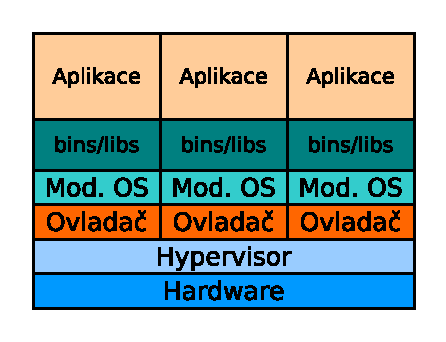
\includegraphics[width=0.8\textwidth]{img/paravirt.pdf}
\par\end{centering}
\caption{Schéma para-virtualizace, zdroj: vlastní tvorba} \label{fig:paravirt}
\end{figure}

\subsection{Plná virtualizace}
Plná virtualizace funguje na principu abstrakce. Všechny fyzické komponenty hostitelského stroje jsou nahrazeny „virtuálním hardwarem“, viz obrázek \ref{fig:fullvirt}. Operační systémy, které fungují na hostitelském počítači nepřistupují přímo na fyzický hardware. Tato skutečnost dává uživateli velké možnosti pro vlastní přizpůsobení virtuálního hardwaru. Vzhledem k této možnosti nejsou aplikace běžící na virtualizovaném systému závislé na fyzicky dostupných komponentech. Další výhodou je fakt, že operační systém, který je použit, nepotřebuje žádné modifikace na rozdíl od para-virtualizace.

\begin{figure}[H]
\begin{centering}
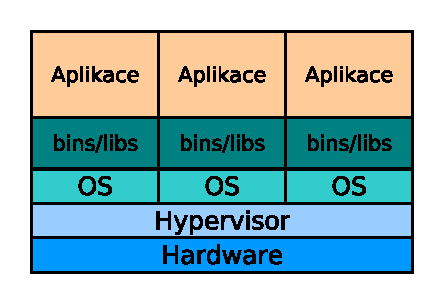
\includegraphics[width=0.8\textwidth]{img/fullvirt.pdf}
\par\end{centering}
\caption{Schéma plné virtualizace, zdroj: vlastní tvorba} \label{fig:fullvirt}
\end{figure}
 
\subsection{Kontejnerová virtualizace}
Kontejnerová virtualizace poskytuje sdílení virtualizačních obrazů operačních systémů skládajících se z root systému, systémových knihoven a spustitelných souborů. Kontejner, poté nahrazuje VM, může být zaveden jako klasický operační systém jenž může být spuštěn, restartován či vypnut. Kontejner může tyto zdroje dynamicky zvýšit či snížit podle potřeby spuštěné aplikace. Aplikace a uživatelé vidí kontejner jako odděleného hosta, znázorněno na obrázku \ref{fig:containervirt}

Kontejnerová virtualizace umožňuje běh jádra s několika odlišnými virtuálními stroji. Na rozdíl od hypervisorové virtualizace nemůže kontejnerový přístup spustit virtuální stroj jako kompletní instanci operačního systému. Kontejnery založené na virtuálních strojích jsou spíše dílčí instance operačních systémů.

Kontejnerová virtualizace nefunguje na celém operačním systému, ale místo toho izoluje systém a nevirtualizuje hardware. Jádro izoluje proces ostatních kontejnerů a řídí jejich zdroje. Všechny kontejnery používají stejné jádro, mají však svůj vlastní file systém, atd.

\begin{figure}[H]
\begin{centering}
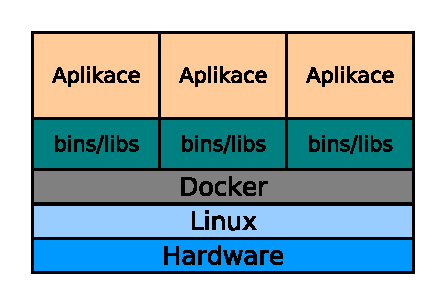
\includegraphics[width=0.8\textwidth]{img/containervirt.pdf}
\par\end{centering}
\caption{Schéma kontejnerové virtualizace, zdroj: vlastní tvorba} \label{fig:containervirt}
\end{figure}

\section{Typy kontejnerové virtualizace}
Kontejnerová virtualizace zažívá obrovský vzestup, spousta firem se snaží kontejnery využít ve svých produkčních prostředích. Rychlý posun kontejnerových technologií v posledních letech lze sledovat převážně díky firmě Docker (původně dotCloud)\cite{dotcloud_docker}. Firma Docker je jedna z firem, která udává směr ve vývoji kontejnerových technologií, a v létě roku 2015 byla oceněna na jednu miliardu amerických dolarů\cite{docker_mil}. 

Kromě technologie od firmy Docker existuje na trhu řada konkurenčních technologií, které z části staví na technologiích Dockeru. Jiné firmy se pokoušejí prosadit se svým vlastním konceptem. S rychlým rozšiřováním kontejnerového trhu přišly obavy o konkurenceschopnost jednotlivých technologií. Technologie Dockeru se objevily na trhu první a mají stále před konkurenčními projekty náskok. Ze strany firem se jedná o technologii, o kterou mají firmy největší zájem, viz obrázek \ref{fig:docker_vs_others}. Podle průzkumu serveru ClusterHQ v roce 2016 jsou kontejnery využívány v produkci v 76 \% dotázaných firem\cite{cluster_vyzkum}.

Díky této skutečnosti vznikla obava, že se z firmy Docker na trhu stane monopol. Z tohoto důvodu byly založeny dvě organizace: OpenContainer Initiative  (OCi) a The Cloud Native Computing Foundation (CNCF). První jmenovaná  je sdružení, které bylo založeno v roce 2015\cite{oci_born} s cílem přinést do kontejnerového světa standardy a dát možnost i jiným firmám podílet se na vývoji kontejnerových technologií, aby všechny kontejnerové projekty měly stejné specifikace pro používané zdroje. CNCF se snaží o větší propagaci kontejnerových technologií a rozšíření se do podvědomí, především v podnikové sféře.

\begin{figure}[H]
\begin{centering}
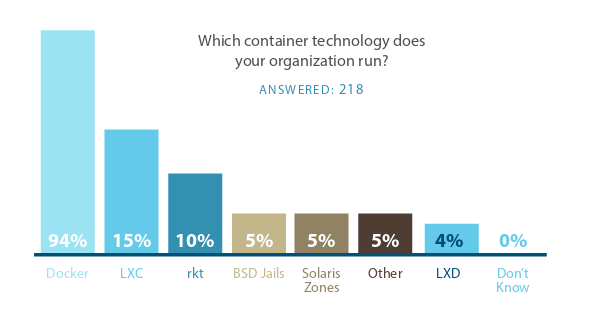
\includegraphics[width=0.8\textwidth]{img/docker_vs_others.png}
\par\end{centering}
\caption{Nejpoužívanější kontejnerové technologie podle serveru ClusterHQ, převzato z \cite{{cluster_vyzkum}}} \label{fig:docker_vs_others}
\end{figure}

V dnešní virtualizaci stále značnou část zastupují VM, avšak mezi technologickými firmami se už VM označují jako legacy technologie. Na rozdíl od klasické virtualizace jsou kontejnery velmi lehkotonážní. Hlavní rozdíl je tak ve smyslu používání. VM můžeme chápat jako celistvý server, na který lze nainstalovat více aplikací a poté obsluhovat více rolí najednou. Ke kontejnerům se musí přistupovat odlišněji. Je potřeba každou službu spustit v odděleném kontejneru a dodržovat tak koncept mikroslužeb. Ve světě kontejnerů je abstrahována celá aplikace. Data produkovaná kontejnerovými aplikacemi nejsou ukládána do kontejnerů ale mimo něj na hostitelský file systém skrze volumy. 


\subsection{Docker}
Docker je platforma zaměřená na kontejnerovou virtualizaci, je publikovaná jako open source, vydaná pod licencí Apache 2.0. Docker není pouze systém, který se zaměřuje na práci s kontejnery. Jedná se o binární balík, který obsahuje i orchestrátory (Compose, Swarm)\cite{docker_1_12}. 

Docker obsahuje nástroje na správu images, pomocí které lze jednotlivé vrstvy image dávat na sebe. Celý koncept images je založen na union mount systému\cite{Docker_OD}. Na obrázku \ref{fig:docker_layers} je znázorněn vrstvící systém, který Docker používá. V tomto vrstvícím systému má pouze vrchní vrstva právo zapisovat, zbytek má pouze právo číst. Tyto images se pak dají šířit pomocí repositáře zvaného Docker Hub, tento repositář funguje na velmi podobném principu jako distribuovaný systém pro správu verzí git. 

Docker je postaven nad ovladačem libcontainer, který ovládá kernel a spravuje systémové zdroje. Libcontainer přišel do Dockeru až s verzí 0.9\cite{docker_lib}, kde nahradil stávající řešení postavené na zdrojích z projektu LXC. Uvnitř Docker kontejneru běží RunC, což je lehkotonážní runtime, který vychází ze standardů OCi. Velkou nevýhodou Dockeru jsou nové verze, které vycházejí nepravidelně každé tři měsíce. Občas se stává, že nová verze není zpětně kompatibilní se starší, tudíž aktualizace je problém zvláště na produkčním prostředí, kde se používají starší a stabilní verze. 

\begin{figure}[H]
\begin{centering}
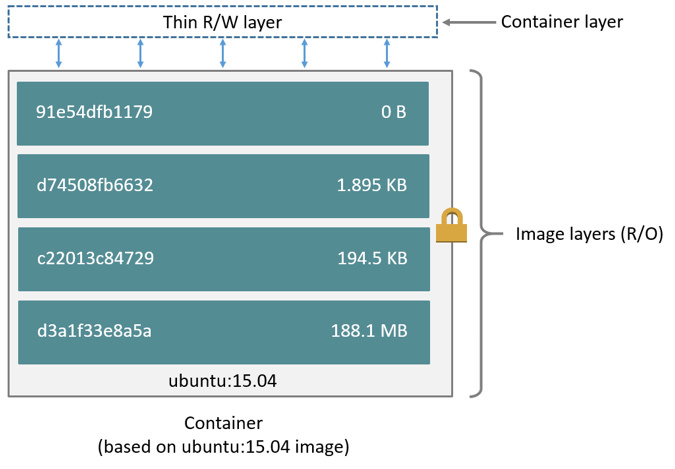
\includegraphics[width=0.7\textwidth]{img/docker_layers}
\par\end{centering}
\caption{Docker vrstvy, převzato z: \cite{Docker_doc_layers} \label{fig:docker_layers}}
\end{figure}

\subsection{Rkt}
Kontejnerová technologie rkt [:rock-it:] je další z řady projektů od firmy CoreOS s otevřeným zdrojovým kódem. Oproti Dockeru rkt není funkční na velkém spektru platforem, nabízí podporu pouze pro Linuxové distribuce. Projekt rkt byl vytvořen a implementuje zmíněné standardy od OCi\cite{coreos_00}. Umožňuje spouštět dva typy images. OCi kompatibilní images vytvořené na základně OCi předpisu a Docker images, které byly vytvořeny konkurenčním řešením. Další odlišnost od konkurenčních řešení je proces model, který dokáže spouštět procesy ve stromové struktuře, je velmi podobný Linuxové struktuře procesů. Rozdíl mezi architekturou Dockeru a rkt je znázorněn na obrázku  \ref{fig:docker_vs_rkt}. 

\begin{figure}[H]
\begin{centering}
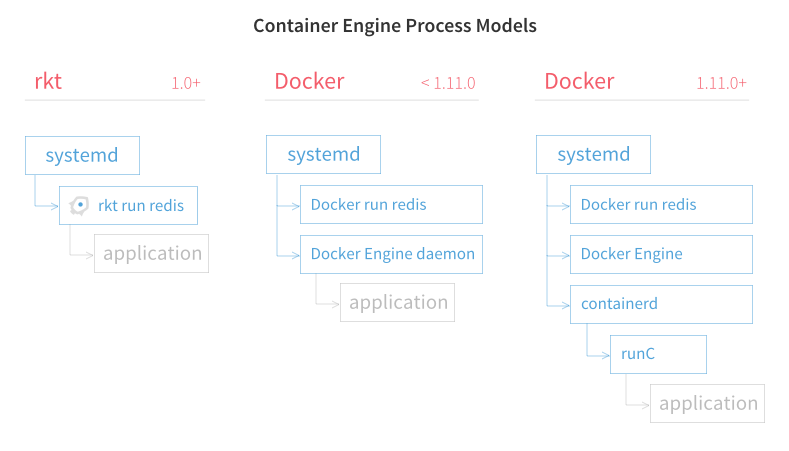
\includegraphics[width=1\textwidth]{img/docker_vs_rkt}
\par\end{centering}
\caption{rkt vs Docker architektura, převzato z: \cite{Docker_vs_rkt} \label{fig:docker_vs_rkt}}
\end{figure}

\subsection{Crio-o}
Cri-o je projekt založený na standardech vytvořených OCi. Zároveň implementuje rozhraní pro kubelet container runtime (CRI). Projekt vzniká pod hlavičkou kubernetes-incubator na serveru github\cite{kube_incubator}. Kubernetes-incubator zastupuje nové projekty, které se týkají Kubernetes a kontejnerů. Projekty nacházející se v incubatoru nejsou na tolik vyspělé, aby mohly být pod oficiální hlavičkou Kubernetes. Projekt Cri-o má stanoven několik hlavních cílů. První z nich je podpora různých typů images založených na standardech OCi. Dalšími jsou managment jednotlivých vrstev těchto images, kontejnerový life-cycle managment a monitorování a správa logů\cite{cri_o_inc}. 

Globální cíl projektu je mít runtime, který umožňuje Kubernetes pomocí CRI implementace spouštět a ovládat kontejnery postavené na standardech od OCi. Cri-o nemá zatím stabilní verzi\cite{cri_o}, takže ho nelze použít v produkčním prostředí.

\section{Výhody kontejnerové virtualizace}
Mezi hlavní výhody patří výkon a škálovatelnost kontejnerů. Hlavní rozdíl mezi kontejnerovou a hypervisorovou virtualizací je, že kontejnery nepoužívají celé VM a mají menší nároky na hardware. Kontejnery běží jako izolované aplikace v rámci operačního systému. Z toho důvodu kontejnerová virtualizace eliminuje potřebu duplikovat určitou funkcionalitu operačního systému, například neduplikuje hardwarová volání a jeden operační systém je zodpovědný za správu všech hardwarových přístupů.
Oproti hypervisorové virtualizaci mají kontejnery limit kolik CPU a paměti bude přiřazeno k operačnímu systému. Kontejnerové řešení by mělo být schopno adresovat všechny volné CPU a RAM paměti pro dané jádro. Vzhledem k tomu, že kontejnery sdílejí operační systém, jsou značně menší než VM. Mohou být tvořeny a spuštěny rychleji než klasická VM. Nabízí tak lepší výkon pro aplikace, které obsahují. Toto řešení je vhodnou volbou, pokud je potřeba nasadit několik desítek až stovek Linuxových hostů.

\chapter{Orchestrace kontejnerů}
Ochestrátory vznikly jako odpověď na rozšiřování kontejnerové virtualizace. Kontejner má stejný problém jako VM, bez orchestrace je práce s nimi velmi zdlouhavá a neefektivní. Na rozdíl od klasické virtualizace se ve světě mikroslužeb pracuje se stovkami tisíc až milióny kontejnerů a tyto objekty je potřeba ovládat. Orchestrátory slouží ke správě a ovládání kontejnerů, pomocí nich lze škálovat, rozdělovat zdroje a řešit spoustu problémů, které by se bez jejich použití musely řešit manuálně. Jak vyplývá z prezentace zaměstnance Google Joe Beda americký internetový gigant Google\cite{beda_prez} spouští během každého týdne cca na 2 miliardy nových kontejnerů. Takové množství nelze spravovat bez orchestrátoru. 

Pro dnešní typy kontejnerů existuje na trhu řada orchestrátorů jejíž vývoj kopíruje vznik Dockeru, ale první stabilní verze 1.0 byly vydávány v letech mezi 2015 a 2016\cite{docker_1_0}. Všechny tyto nástroje jsou taktéž jako kontejnerové technologie open source.

Orchestrátory fungují na jednoduchém principu, rozdělují jednotlivé kontejnery do logických skupin a pracují se skupinou samostatně, například  skupina pro webové servery, databáze atd. Díku tomuto faktu lze pak s logickou skupinou pracovat jako s jedním kontejnerem. Například v případě potřeby přidání  storage se připíše její definice pouze k předpisu pro tuto skupinu a orchestrátor zajistí, že všechny kontejnery dostanou potřebné místo.

Networking v rámci orchestrátorů je velmi odlišný od Docker networkingu. Každý orchestrátor má v základu své řešení, které většinou dovoluje komunikovat veškerým kontejnerům navzájem mezi sebou, což není optimální ve všech případech. Pokud běží na jedné infrastruktuře více odlišných aplikací, pak je nutno omezit jejich viditelnost. Problémy, které jsou v rámci síťování potřeba vyřešit jsou následující: komunikace mezi kontejnery, viditelnost vůči externímu světu a vysoká dostupnost\cite{K8S_micro}. Podobně, jak je tomu u klasické virtualizace, existují i projekty od externích firem, které rozšiřují a vylepšují základní koncept networking u orchestrátorů a přidávají spoustu nových funkcí (OpenContrail, Calico, Romana, apod.).

Pro nasazení kontejnerů v produkčním prostředí je potřeba vyřešit ještě mnoho důležitých otázek a požadavků, které jsou od těchto prostředí vyžadovány. Spousta vlastností jako vysoká dostupnost či life cycle managment nejsou pouze o vybrané technologii, ale i o designu daného prostředí. Pokud je navrženo špatně, tak vybrané technologie nemohou být využity efektivně. 

\section{Vysoká dostupnost} \label{par:ha}
Pojem vysoká dostupnost (v angličtině High Avalibility) popisuje proces, pomocí kterého se udržuje infrastruktura dostupná pro uživatele. Pokud má infrastruktura tento prvek správně navržený, koncový uživatel by neměl poznat žádný problém způsobený například pádem databáze nebo webového serveru. Faktor vysoké dostupnosti bývá někdy podceňován, nejedná se totiž jenom o infrastruktru, ale i o datacentra, kde se daná infrastruktura nachází. Vysoká dostupnost závisí na čtyřech hlavních kategoriích hardwaru, sítí, storage a používaného softwaru. Cílem vysoké dostupnosti je omezit tzv. single point of failure, jedná se o jednu část, například službu, při jejímž výpadku by mohlo dojít k poruše celého prostředí.

Řešení problému single ponint of failure probíhá pomocí mnoha procesů, které slouží jako prevence před případným výpadkem prostředí. Důležité je duplikovat služby a pokud je to možné, provozovat je v cluster módu, aby případný výpadek jedné komponenty v clusteru nemohl ovlivnit zbytek. Velmi důležitou částí v tématu vysoké dostupnosti hrají load balancery, které slouží pro rozložení zátěže mezi více odlišných a na sobě nezávislých komponent, například webserver, viz obrázek \ref{fig:load_balancing}. Je potřeba zmínit, že pokud se na produkční prostředí přistupuje prostřednictvím load balanceru, je nutné vytvořit z load balancerů cluster, a tím zamezit případným výpadkům prostředí.

\begin{figure}[H]
\begin{centering}
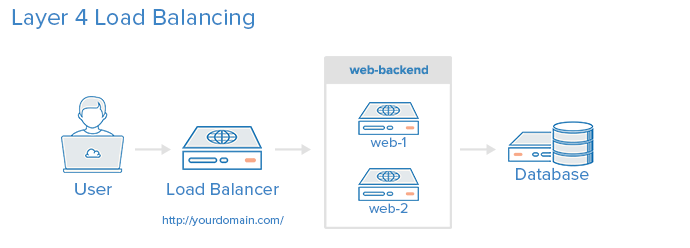
\includegraphics[width=1\textwidth]{img/load_balancing}
\par\end{centering}
\caption{Ukázka architektury Load Balanceru, převzato z: \cite{lb_ha} \label{fig:load_balancing}}
\end{figure}

V produkčním prostředí jsou požadavky na dostupnost služeb velmi vysoké, proto je nutno aplikovat pravidla pro vysokou dostupnost. Pomocí implementací principu vysoké dostupnosti lze minimalizovat výpadky v prostředí. Moderní programy zaměřující se na řešení vysoké dostupnosti provádějí i automatické obnovy ze záloh serveru či dokonce obnovu chybných komponent v clusteru. 

\section{Škálovatelnost}
Dalším faktorem, který je nutno při výběru orchestrátoru třeba zvážit, je škálovatelnost neboli schopnost rozšiřovat dané prostředí. V dnešní době se stává, že firmy rostou několikanásobně za rok. V důsledku přibývajících uživatelů a jejich potřeb je nutno škálovat a rozšiřovat dané služby tak, aby byla uspokojena uživatelská poptávka. S tímto problémem se například potýká největší poskytovatel streamované hudby na světě server Spotify.
Ve škálovatelnosti jsou definovány dva základní druhy škálování, a to horizontální a vertikální. Vertikální prostředí můžeme chápat jako přidávání dalších zdrojů pro hardware, přidávání disků a rozšiřování RAM. Škálování horizontální je rozšiřování daných služeb na jedné infrastruktuře.

Orchestrátory umí škálovat pouze horizontálně. Hlavním parametrem škálovatelnosti je čas, za který orchestrátor vytvoří nové kontejnery, a tím zvýší dostupnost stávajícím službám. Obdobný princip funguje i obráceně. Pokud není potřeba zpracovávat velké množství dat od koncových uživatelů, je možno kontejnery s těmito nepoužívanými aplikacemi jednoduše zastavit. 

Ochestrátory mohou provádět škálování kontejnerů automaticky podle nastavených specifik, prostředí se  automaticky přizpůsobuje potřebám aplikací a není tak nutný manuální zásah administrátorů přímo do prostředí.

\section{Life cycle managment}
Life cycle managment (LCM) je založen na řadě procesů, které slouží  k udržování a běhu aplikace po dobu produkce. Infrastruktura je živé prostředí, ve kterém je doporučeno uchovávat a spravovat konfigurační soubory.
V rámci automatizace těchto kroků vznikla nová sada nástrojů spadající do skupiny konfigurační management. Pomocí těchto nástrojů lze vzdáleně přes jeden server ovládat stovky až tisíce serverů. Mezi tyto nástroje patří Ansible, Puppet, SaltStack, Chief atd.
Globální konfigurační soubory je vhodné ukládat přes distribuovanou službu, například git. Konfiguraci je  vhodné verzovat a mít tak možnost vrátit se ke starším verzím konfiguračních souborů. Užitečná vlastnost na verzovacích nástrojích je kontrola změn. Všechny verze se změnami konfigurace se ukládají do repositářů. Pokud je repositář, ve kterém jsou uloženy konfigurační soubory správně nastaven, není možné, aby nikdo z administrátorů, který upravuje konfiguraci, změnil historii repositáře. Další výhodou těchto nástrojů pro distribuovanou správu verzí je indexování změn.
V LCM je velmi důležité téma aktualizace stávajících aplikací běžících v kontejnerech. V rámci prudkého vývoje aplikací je velmi důležité nasazení nové verze do produkce velmi rychle. 

\section{Typy orchestrátorů}
Na trhu existuje mnoho projektů na správu kontejnerových prostředí. Tato práce se zaměřuje na pět základních druhů. Orchestátory se převážně liší svým přístupem a ovladatelností, ne všechny jsou vhodné jako produkční orchestrátory ve velkých infrastrukturách. U jednotlivých technologií je rozhodující počet kontejnerů, se kterými orchestrátor dokáže pracovat.

\subsection{Docker Compose}
Compose je řešení od firmy Docker, které zajišťuje spouštění multi-kontejnerových Docker aplikací. Lze ho označit jako jednoduchý orchestrátor. Na rozdíl od ostatních řešení nabízí poměrně málo funkcionality. Hlavním stavebním kamenem služby Compose je konfigurační yml dokument, pomocí kterého se nastavuje spojení mezi jednotlivými kontejnery. Do logických bloků se nadefinují potřebné údaje jako jsou image, volume, které je pro dané prostředí nutné nastavit. Vzorová ukázka Docker Compose souboru v yml formátu se nachází v ukázce kódu číslo \ref{lst:compose_code}.  Dalšími přednostmi yml je čitelnost a přehlednost, která je u formátu json  horší. 

Velká přednost, a zároveň nevýhoda tohoto řešení, je jeho jednoduchost. Tento koncept je spíše použitelný zejména pro vývojáře, kteří si mohou pomocí Compose spustit jednoduché vývojové prostředí s předem nadefinovanými službami (databáze, webserver, apod.). Compose vůbec neřeší problém jako jsou vysoká dostupnost, distribuovanost a LCM, proto není vhodný pro velké infrastruktury.  

\begin{lstlisting}[caption={Docker Compose pro Wordpress s MySql databází},label= {lst:compose_code}]
version: '2'
services:
   db:
     image: mysql:5.7
     volumes:
       - db_data:/var/lib/mysql
     restart: always
     environment:
       MYSQL_ROOT_PASSWORD: wordpress
       MYSQL_DATABASE: wordpress
       MYSQL_USER: wordpress
       MYSQL_PASSWORD: wordpress

   wordpress:
     depends_on:
       - db
     image: wordpress:latest
     ports:
       - "8000:80"
     restart: always
     environment:
       WORDPRESS_DB_HOST: db:3306
       WORDPRESS_DB_PASSWORD: wordpress
volumes:
    db_data:
\end{lstlisting}

\subsection{Fleet}
Fleet je další z projektů od firmy  CoreOS. Je založen na systemd. Systemd nyní používá většina Linuxových distribucí jako init a pomocí něj spravuje procesy\cite{fleet_systemd}. Fleet by se dal nazvat jako systemd pro cluster, který si udržuje data v distribuované databázi etcd. Tento projekt směřuje primárně na linuxovou distribuci od firmy CoreOS Container Linux. Práce s clusterem je jednoduchá, velmi podobná práci se systemd samotným. Samostatné používání tohoto orchestrátoru na velkém produkčním prostředí je trochu limitující, sami autoři projektu nedoporučují použít Fleet na více jak 100 serverech s více než 1000 službami\cite{fleet_lim}. V únoru 2017 firma CoreOS pozastavila vývoj uvedeného orchestrátoru a začala ve všech svých produktech používat Kubernetes\cite{fleet_end}. 

\subsection{Docker Swarm}
Swarm je nástroj pro tvorbu clusteru pro Docker kontejnery. Původně byl doručován jako doplněk k Docker kontejnerům. Od verze Dockeru 1.12 byl přidán do stejného balíku\cite{docker_1_12}, ve kterém je doručováno kontejnerové řešení. V tomto novém řešení přišel s vlastnostmi a architekturou velmi podobnou konkurenčnímu řešení Kubernetes, viz obrázek \ref{fig:swarm_arch}. Swarm má k dispozici vlastnosti jako rolling update, decentralizovaný design, multi-host networking, load balancing. Jednou z výhod tohoto řešení je nativní podpora pro spouštění již předvytvořených Compose souborů\cite{swarm_compose}. 

V porovnání s Compose se jedná už o vyspělejší řešení podobné ostatním orchestrátorům. Nabízí v základu mnoho vestavěných funkcí. Jeho možnosti jsou stále omezené ve srovnání s komunitou a ekosystémem okolo Kubernetes. Swarm řešení je vhodné pro malé clustery, je velmi jednoduché na operování, nasazení a použitelné v malých produkčních prostředích. Jednou z limitací  orchestrátoru Swarm je rozšiřitelnost, dokáže pracovat pouze s Docker kontejnery. 


\begin{figure}[H]
\begin{centering}
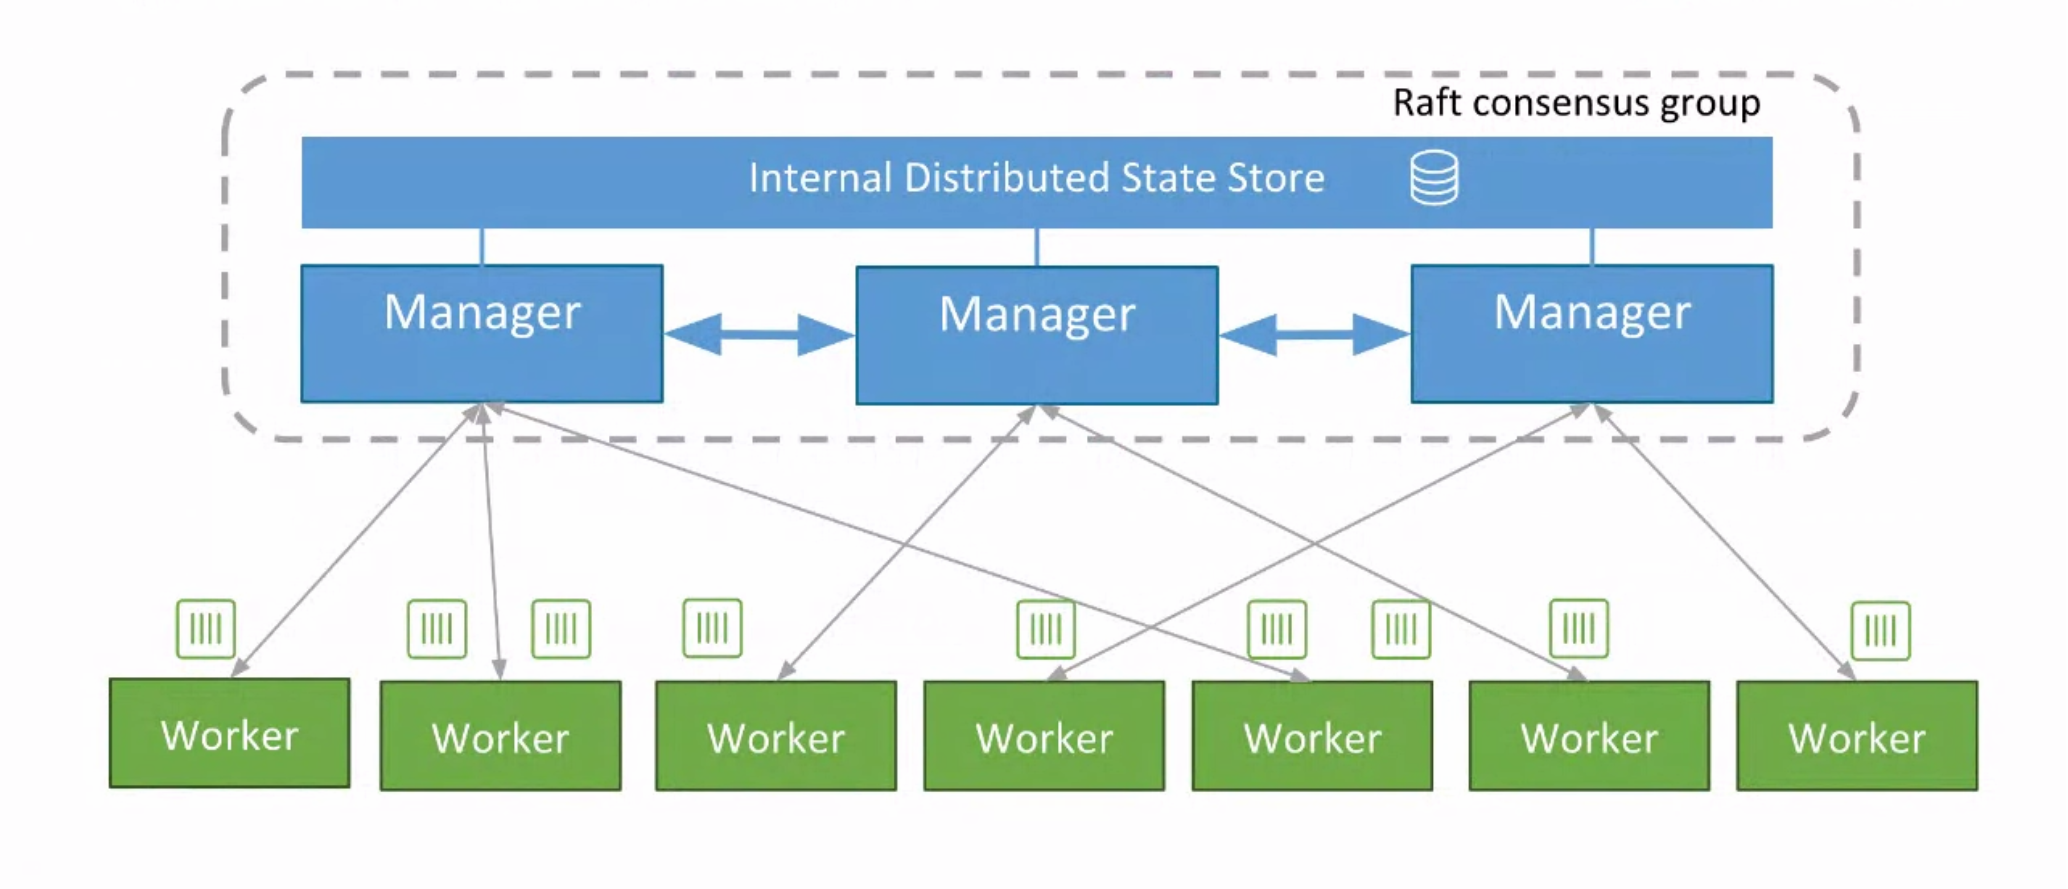
\includegraphics[width=1\textwidth]{img/swarm_arch}
\par\end{centering}
\caption{Docker Swarm architektura, převzato z: \cite{swarm_arch} \label{fig:swarm_arch}}
\end{figure}

\subsection{Apache Mesos}
Apache Mesos je projekt, který se zabývá problematikou distribuovaných clusterů. Od ostatních orchestrátorových řešení se Mesos liší tím, že se nezaměřuje pouze na kontejnery. Pracuje převážně s hardwarovými zdroji, byl vytvořen už v roce 2009 na Univerzitě v Berkeley v Kalifornii\cite{mesos}, a to o tři roky dříve než se začaly objevovat první verze kontejnerů od Dockeru. Je sestaven převážně z projektů pocházejících z Apache Foundation, viz obrázek \ref{fig:mesos_arch}. Jedná se o open source řešení.

Hlavní odlišností od Kubernetes a Swarmu je dvou-úrovňový scheduler, který na první vrstvě pracuje se zdroji pomocí různých typů labelů. Jimi lze odlišovat a spojovat do skupiny různé tipy hardwarových zdrojů. Na druhé vrstvě scheduleru Mesos rozděluje zdroje mezi zdrojové frameworky a frameworky s technologií běžící v nich. Na spouštění kontejnerů pak slouží Marathon framework.

Tento orchrestrátor se často porovnává s open source řešením pro cloud computing OpenStack. Mesos také bývá používán na řešení problematiky velkých objemů dat. 

\begin{figure}[H]
\begin{centering}
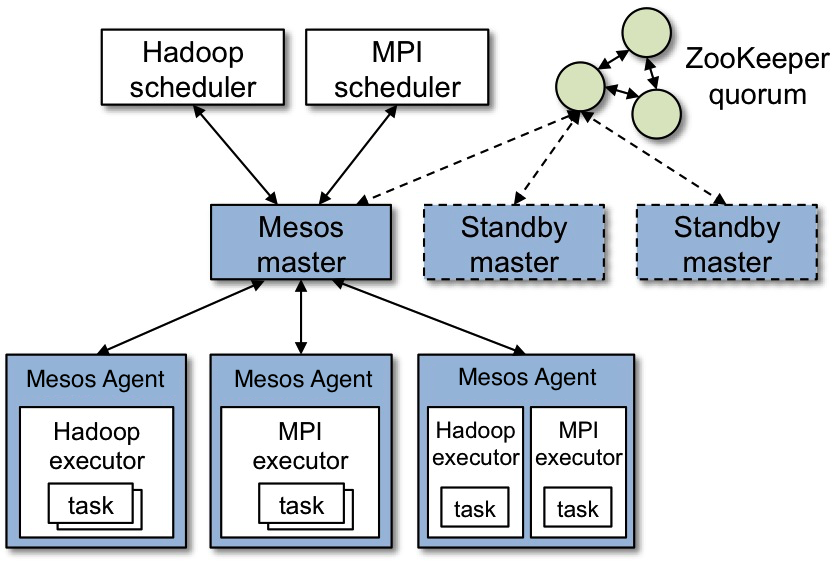
\includegraphics[width=1\textwidth]{img/mesos_arch}
\par\end{centering}
\caption{Mesos architektura, převzato z: \cite{mesos} \label{fig:mesos_arch}}
\end{figure}

\subsection{Kubernetes}
Projekt Kubernetes pochází od firmy Google, tato americká firma používá v produkčním prostředí výhradně kontejnerové technologie\cite{beda_prez}. Všechny jejich webové služby jsou spuštěny v tomto typu virtualizace. Kubernetes je orchestátor, který na rozdíl od ostatních technologií podporuje více kontejnerových řešení. Dokáže pracovat s většinou kontejnerových technologií, jako je Docker, rkt, crio-o, Windows kontejnery atd. Kubernetes by se dal nazvat spíše frameworkem než orchestrátorem, je na rozdíl od ostatních řešení velmi modulární a existuje pro něj celá řada rozšiřujících modulů\cite{k8s_kuba}. 

Kubernetes umožňuje spouštět a spravovat kontejnery, nezávisle na hardware Kuberenetes si sám vybírá místo pro spuštění kontejnerů. Podobně jako u Mesosu řadí všechny fyzické zdroje do jednoho celku, ze kterého si podle potřeby postupně alokuje zdroje. 

Kubernetes se skládá ze dvou základních rolí, master a node (dříve nazýván minion). Master je hlavní součást, která kontroluje jednotlivé skupiny nodů. Nody přebírají požadavky od mastera a vykonávají  akce stanovené masterem. Na základně provedené akce vracejí masterovi zpětnou vazbu o výsledku provedené akce. Kubernetes pro spouštění a správu kontejnerů používá tři základní komponenty: pod, replication controller a Kubernetes services a kubelet viz obrázek \ref{fig:kube_arch}.

Pod je základní stavební jednotka Kubernetes. Jednotlivé kontejnery jsou umísťovány do těchto na sobě nezávislých podů, které nejsou závislé na hostiteli. Do jednoho podu je možno uložit celou aplikaci, která se skládá z více na sobě závislých kontejnerů. Velká výhoda toho konceptu je následná práce s pody, se kterými lze pracovat jako s celistvým objektem. K podu lze připojovat různé zdroje, které mohou kontejnery uvnitř sdílet. 

Replication controller hlídá a definuje pody. V Kubernetes se používá při horizontálním škálování. Další důležitá funkcionalita replication controlleru je hlídání stávajících podů a kontejnerů v nich. V případě výpadku podů nebo výpadku hostitelského stroje, na kterém pod pracuje replication controller je schopen zmonitorovat a spustit nový pod na jiném hostu. V případě, že je chyba na jednom hostu, jsou všechny jeho pody spuštěny na jiném stroji. Pokud je původní host obnoven, pody se opět vrátí na původní místo a stávající pody jsou zrušeny.

\begin{figure}[H]
\begin{centering}
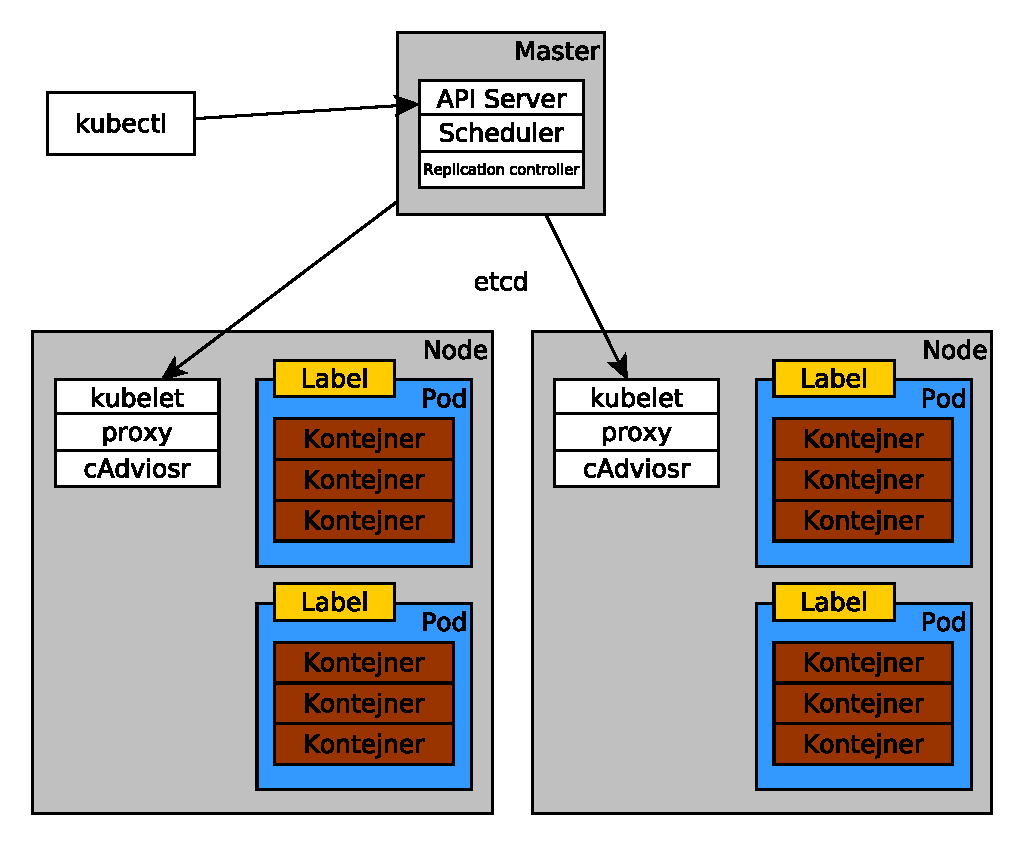
\includegraphics[width=1.0\textwidth]{img/kubernetes}
\par\end{centering}
\caption{Kubernetes architektura, zdroj: vlastní tvorba \label{fig:kube_arch}}
\end{figure}

\section{Porovnávání orchestrátorů}
Z porovnání jednotlivých orchestračních nástrojů lze vysledovat, že většina z nich implementuje maximálně dvě řešení pro spouštění odlišných tipů kontejnerů. Všechny orchestátory až na fleet lze spustit na odlišných platformách, nutno zmínit, že nativní podporu má pouze Linux. Konkurenční platformy jako Mac a Windows lze využít pouze na testování nebo vývoj aplikací pro tyto orchestátory. Škálovatelnost jako hlavní prvek a účel orchestrátoru je podporována napříč všemi vybranými řešeními.  Postupy pro řešení failoverů a vysoké dostupnosti jsou implementovány taktéž u většiny řešení. Pokud je nutné pro orchéstrátor využít externí rozšiřující doplňky pro síťování, je výběr velmi omezen. Tuto funkcionalitu podporují pouze tři řešení, z toho Docker Swarm, podporuje jen jednoduchá SDN. Pokročilé SDN nástroje jako OpenContrail, pomocí kterých lze Kubernetes integrovat do stávajících virtualizačních platforem jako je OpenStack jsou dostupné pouze pro Mesos a Kubernetes. Srovnání orchestrátorů je uvedeno v tabulce \ref{tbl:orch_comp}.

\begin{table}[H]
\begin{center}
\caption{Porovnání orchestrátorů}
\label{tbl:orch_comp}
\begin{tabular}{|c|c|c|c|c|c|}
\hline
  ~   & Compose & Swarm & Fleet & Mesos  &  Kubernetes \\    \hline
Kontejnery          &  Docker &  Docker & Docker, rkt &  Docker, rkt &  \makecell{ Docker, rkt,\\cri-o, \\Windows Containers}  \\    \hline
Škálovatelnost &  Ano &  Ano & Ano &   Ano & Ano \\    \hline
Failover &  Ne & Ano & Ano &  Ano & Ano \\    \hline
Vysoká dostupnost &  Ne  &  Ano & Ano &   Ano & Ano \\    \hline
Netowkring pluginy &  Ne &  Ano & Ne &   Ano & Ano \\    \hline

\end{tabular}
\end{center}
\end{table}


\chapter{Analýza aplikace ve standardním podnikovém prostředí}
Aby aplikace byla v kontejnerovém prostředí škálovatelná, musí zároveň být distribuovatelná. Některé dnešní aplikace bohužel nelze převést do kontejnerů z důvodu špatné práce s pamětí. Tyto aplikace si uchovávají data v paměti a ukládají se na disk, až se aplikace zastaví. Migrovaná aplikace by měla být bezstavová.   

Aplikace je možné rozdělovat podle několika faktorů. Jedním z nich je stavovost, stavy definují jak služby a uživatelé komunikují se serverem. Z počátku většina webových aplikací byla bezstavová, jednalo se totiž o statické stránky, které měly velmi omezené možnosti interakce s koncovým uživatelem. S rozšířením webu se začal měnit přístup k webovým aplikacím na stavový model.

\section{Stavové aplikace (statefull)}
Stavová aplikace je taková aplikace, která udrží po dlouhou dobu otevřené spojení buď k uživateli, nebo k další službě. Pro tento typ aplikací musí být přizpůsobena řada komponent v infrastruktuře například databáze, webové servery, apod. Stavové aplikace jsou nejčastějším typem aplikací nacházejících se v podnikovém prostředí. Tyto aplikace musí mít striktně nastavené hostitelské prostředí, kde běží. Jejich největším problémem je špatná dynamika způsobená velkým množstvím závislostí na jednotlivých komponentách. Jeli aplikace vytížená, není ji možné škálovat a replikovat díky uchovávání stavů. Největší problém se škálováním je u databází .

\section{Bezstavové aplikace (stateless)}
Bezstavový přístup k aplikacím je vlastnost, která je v kontejnerovém světě zcela běžná. Díky této vlastnosti lze jednotlivé aplikace efektivně škálovat a šířit napříč vybranými platformami. Hlavní podstatou toho principu je přístupnost a komunikace mezi jednotlivými službami. Například: všechna data, se kterými aplikace pracují, by měla být ukládána v databázi, do které se aplikace bude připojovat. Databáze by neměla být závislá jen na jedné aplikaci, ale na celé řadě replik, které se vytvoří při škálování. 

Kontejnery jsou pouze jednotky, které vykonávají jednu činnost a neobsahují žádná data, proto bezstavový přístup povoluje kontejnerům nejen škálování, ale také rychlé vypínání a zapínání. Stavové aplikace jsou zejména doménou starého principu virtualizace, kdy se pro každou službu spouštěl jeden VM. Tyto aplikace bývají rovněž označovány jako legacy. Porovnání stavových a bezstavových architektur je na obrázku číslo \ref{fig:arch_app_statefull}.

\begin{figure}[H]
\begin{centering}
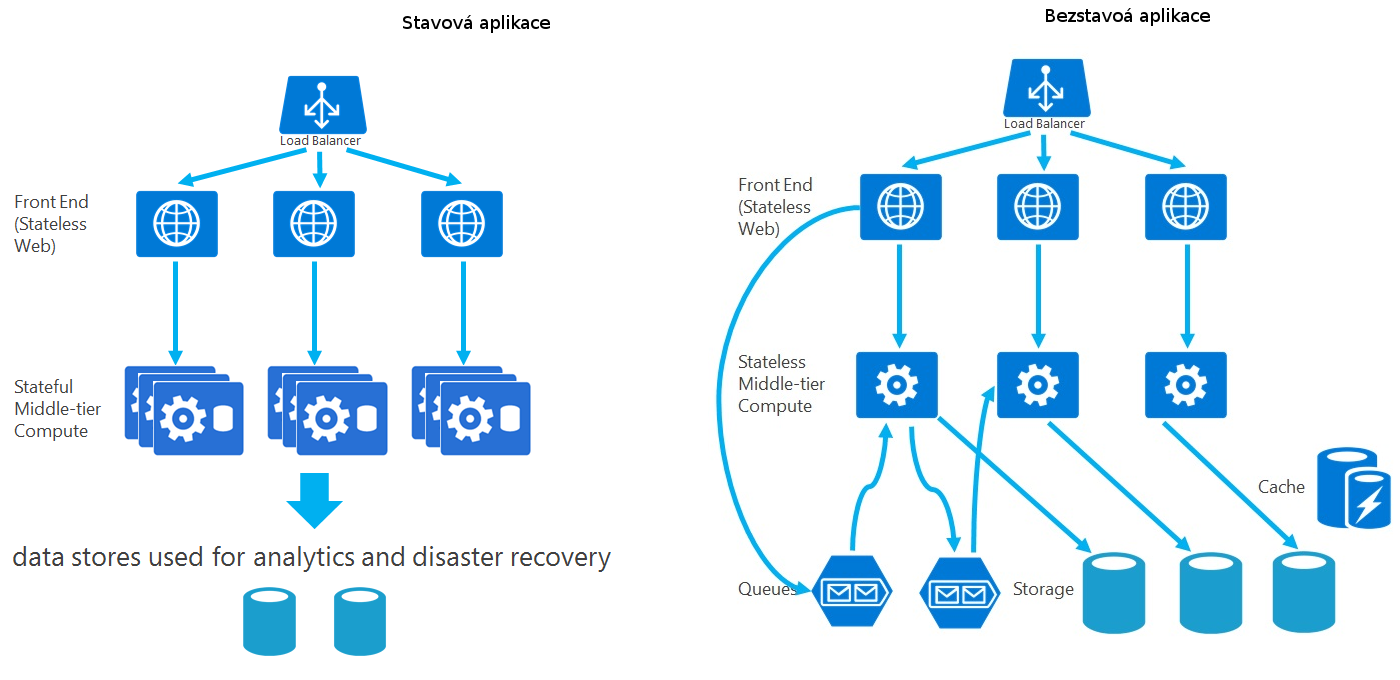
\includegraphics[width=1\textwidth]{img/micro_statefull}
\par\end{centering}
\caption{Rozdíl mezi stavovou a bezstavou aplikací z: \cite{ms_ms} \label{fig:arch_app_statefull}}
\end{figure}

\section{Architektura nekontejnerových aplikací}
Hlavní rozdíl mezi kontejnery a klasickým VM je v práci se zdroji. Tento problém byl již vysvětlen v kapitole číslo \ref{chp:kontejner}, nyní je třeba se zaměřit na architekturu aplikací běžících ve VM. Většina těchto nekontejnerových aplikací používá stavový přístup k datům. Služby tak nejsou specificky odděleny, například proxy server s sebou může nést více rolí z důvodu šetření zdrojů. Pro zachování principů vysoké dostupnosti musí být i VM přizpůsoben tak, aby při chybě na infrastruktuře aplikace fungovala i nadále. K tomu je nutné používat principy popsané v části \ref{par:ha} o vysoké dostupnosti. Problém se zdroji u VM je v jejich alokaci. Při spuštění VM se nastaví určité parametry, jako je počet jader, ram, hdd, a s těmito zdroji nelze dynamicky a efektivně pracovat. Většina virtualizačních technologií umí v reálném čase přidávat a snižovat tyto zdroje, ale samotné zvyšování znatelně ubírá výkon celému VM. Proto je vhodné alokovat pro dané VM dostatečné množství zdrojů a měnit je pouze v kritických situacích. Tím se běžně stává, že na serverech běží VM, které značně plýtvají se zdroji, protože je nedokáží plně využít.

\section{Popis aplikace}
Migrovaná aplikace v této práci je webová aplikace. V aplikaci byly použity komponenty Nginix, Memcached, MySql a OwnCloud. Celé schéma aplikace v kontejnerovém prostředí je zobrazeno na obrázku \ref{fig:arch_app_statefull}

Nginx je open source řešení pro webový server a reversní proxy. Koncept technologie Nginx je postaven na rychlé distribuci statického obsahu. Na rozdíl od Apache (webový server od Apache Foundation) vyřizuje všechny požadavky asynchronně. Mnohem častěji je však Nginx používán jako proxy server, který slouží například při přístupu z internetu do vnitřní sítě. Pomocí Nginxu lze nastavit řadu dalších nastavení, jako jsou limity připojených uživatelů na danou adresu, http/https redirecty, filtrace přístupů podle dané lokace atd. Nginx je jeden z nejrozšířenějších nástrojů pro web server/proxy na světě, využívají ho firmy jako Seznam.cz, Github či Dropbox\cite{ngnix}. 

Memcached je distribuovaný cache systém. Distribuovaná cache řeší problém při potřebě vyřídit požadavky při velkému přístupu uživatelů, díky tomuto řešení není potřeba upravovat část kódu aplikace či dokonce přidávat další hardware. Toto řešení je velmi podobné konkurenčnímu redisu, který je v praxi mnohem více rozšířen pro jeho jednoduchost. Hlavní důvod pro volbu memcached byla jeho multi-threadová podpora oproti redisu který dokáže pracovat pouze s jedním threadem. 

MySql je jedno z nejrozšířenějších open source řešení pro relační databáze. Velkou předností MySql je schopnost spouštění tohoto databázového řešení na všech dostupných platformách. Databáze se ovládá pomocí jazyka SQL. Mezi další výhody tohoto databázového řešení patří vysoká rychlost, jednoduché zálohovaní, apod. 

  %https://sysdig.com/blog/sysdig-docker-usage-report-2017/
Jako hlavní aplikace, která stojí mezi těmito open source projekty, byl zvolen OwnCloud. Owncloud je jednoduchá webová aplikace napsaná v programovacím jazyce PHP. Tato aplikace se zaměřuje na sdílení dat. OwnCloud je velmi podobný službám jako Google Drive, Dropbox. Hlavní výhodou je jeho otevřenost, díky otevřenému kódu řada vývojářů doimplementovala nové vlastnosti, jako jsou kalendáře, úprava tabulek a textových dokumentů, poznámky apod. Pro obsluhu OwnCloudu také lze používat mobilní aplikace, které byly oficiálně vydané firmou OwnCloud. 

Nevýhodou OwnCloudu je jeho oficiální podpora. Během minulého roku firmu opustila většina klíčových vývojářů, kteří si vytvořili nový projekt NextCloud (fork OwnCloudu). Podpora tohoto projektu tak zůstává převážně na komunitě uživatelů.


\begin{figure}[H]
\begin{centering}
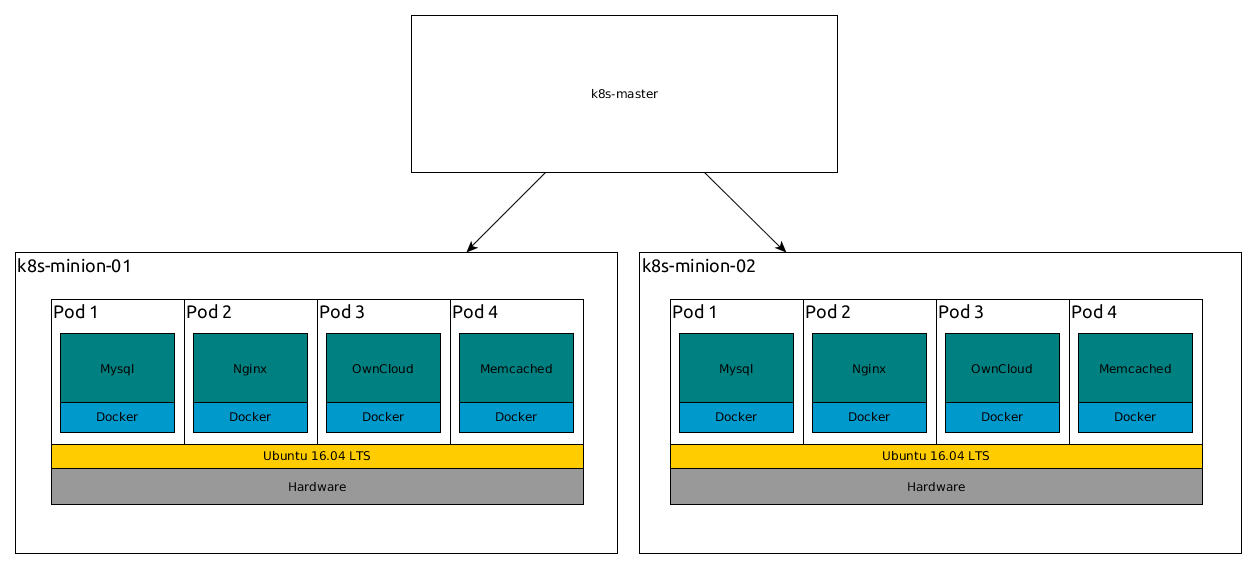
\includegraphics[width=1\textwidth]{img/k8schema}
\par\end{centering}
\caption{Architektura aplikace v kontejnerovém prostředí aplikací, zdroj: vlastní tvorba \label{fig:k8schema}}
\end{figure}


\section{Vybrané technologie}
V druhé a třetí kapitole byly představeny koncepty orchestrátorů a kontejnerů. Ve výběru je zohledněn faktor modularity a nahraditelnosti daného řešení. Každá infrastruktura měla být stavěna modulárně, aby bylo možno vyměnit jednotlivé komponenty bez větších změn.

\subsection{Kontejnerová technologie}
Pro kontejnerovou technologii je v práci použita technologie Docker, která je bezkonkurenčně nejrozšířenější. Byla zvolena převážně díky jednoduché tvorbě nových kontejnerů a díky snadnější práci s vrstvícím systémem. Další výhodou je vestavěný systém na práci s images, který Docker implementuje. Zároveň lze velmi jednoduše propojit s repositářem po ukládání těchto images.
Výhodou Docker images je jejich znovupoužitelnost. Jakmile je image sestavený, lze ho volně převést na rkt kontejner. Pro kompatibilitu lze také využít rkt runtime, který dokáže rovněž spouštět a provozovat Docker kontejnery. 

\subsection{Orchestátor}
Pro praktickou část je zvolen orchestártor Kubernetes. Splňuje všechny požadavky, jako jsou vysoká dostupnost, škálovatelnost a life-cycle-management. Jelikož praktická část je zaměřena především na modularitu, výběr byl omezen pouze na orchestrátory Mesos a Kubernetes. 

Mesos nebyl zvolen, protože se jedná o nástroj, který není zaměřen pouze na kontejnery a pro jeho instalaci je důležité vyřešit spoustu dalších otázek (například nastavení zookeeperu). Tento nástroj je vhodné řešení zejména pro celá datová centra, kde dokáže efektivně řídit zdroje. Pro potřeby menších clusterů je příliš těžkopádný a složitý.

Kubernetes ve své architektuře implementuje postupy, které by se mohly nazývat automatické léčení (self-healing). Orchestrátor dokáže ve stanoveném čase reagovat na podněty, jako jsou pády kontejnerů a služeb. V případě poruchy je schopen obnovit chybějící části aplikace na jiné části infrastruktury. Všechny tyto operace se mohou provádět především díky  distribuované architektuře Kubernetes. 

Rozšiřitelnost stávajícího clusteru je také důležitý prvek, ve velkých systémech je nežádoucí, aby přidávání nového hardwareru bylo složité a zdlouhavé. V Kubernetes rozšiřování funguje velmi jednoduše, stačí na daném zařízení nastavit roli, kterou má vykonávat, a předat informaci o novém serveru Kubernetes masteru. Všechny dodatečné procesy jako adresování a spouštění nových kontejnerů si Kubernetes určí sám. 

\chapter{Migrace aplikace do kontejnerové virtualizace}
Kubernetes je funkční napříč různými platformami, od cloudu až po bare matel. V této práci je orchestrátor Kubernetes nainstalován přímo na fyzické servery, jejichž specifikace jsou uvedeny v tabulce \ref{tbl:hp_hardware}. Na všech serverech je nainstalován operační systém Ubuntu 16.04 pomocí open source nástroje Ubuntu MAAS.

\begin{table}[H]
\begin{center}
\caption{HW konfigurace HP serverů}
\label{tbl:hp_hardware}
\begin{tabular}{|l|l|}
\hline
\textbf{CPU} & Intel(R) Xeon(R) CPU E3-1231 v3 @ 3.40GHz (8 jader)\\
\hline
\textbf{RAM} & 32GB(4x 8GB) ECC DDR3 1600MHz \\
\hline
\textbf{HDD} & 2000GB (2x 1TB)  SATA 3.5" \\
\hline
\textbf{OS} & Ubuntu 16.04 LTS "Xenial Xerus" \\
\hline
\end{tabular}
\end{center}
\end{table}


\section{Instalace Kubernetes}
Jedním z důležitých faktorů je volba nástroje, pomocí kterého je Kubernetes cluster nainstalován, na trhu existuje celá řada takových nástrojů určených k instalaci. Tato řešení bývají většinou postavena okolo nástrojů na konfigurační management. Kubernetes cluster a kontejnery jsou prostředí, která jsou potřeba během používání řídit. Při výběru instalačního nástroje je také vhodné vyzkoušet, jakým způsobem  pracuje nástroj s koncepty LCM a jak je pomocí něj schopen řešit aktualizace samotného Kubernetes.

V této práci byl pro instalaci zvolen nástroj kargo, který se nachází pod hlavičkou kubernetes-incubátoru. Předností tohoto projektu je použití a implementace, je možné jej využit na instalaci Kubernetes clusteru napříč širokým spektrem cloudových prostředí, jako jsou AWS, GCE, OpenStack atd. Instalační nástroj kargo je postaven nad konfiguračním nástrojem Ansible, jeho použití je velmi jednoduché. Pro instalaci lze využít buď nástroj kargo-cli nebo přímo Ansible playbook s definicí pro cluster. Z důvodu nefunkčnosti nástroje kargo-cli je pro tuto práci zvoleno druhé řešení, instalace pomocí playbooku.

V rámci této práce není důležitá podrobná analýza karga. Pro demonstraci instalace stačí pouze inventory soubor, viz překlad kódu \ref{lst:kargo_invenotry}, do kterého je potřeba vyplnit ip adresy serverů a zvolit jednotlivé role. Pokud není při instalaci specifikováno síťové řešení, je kargo nainstalované s projektem Calico, což je jednoduché SDN řešení.

\begin{lstlisting}[caption={Inventory soubor pro Kargo},label={lst:kargo_invenotry}]
[kube-master]
10.0.175.86

[etcd]
10.0.175.86

[kube-node]
10.0.175.85
10.0.175.84
10.0.175.83

[k8s-cluster:children]
kube-node
kube-master
\end{lstlisting}

Po správném vyplnění inventory souboru stačí jen spustit daný Ansible playbook. \textit{Ansible-playbook -i inventory/inventory.cfg cluster.yml}.
Pokud není specifikován atribut flag \textit{-u} pro uživatele, Ansible se automaticky napojí na uživatele root. A po ssh se začne spojovat s ostatními servery a aplikovat proces nadefinovaný v Anible playbook. Užitečná vlastnost těchto konfiguračních nástrojů je idempotentnost. Pokud je přidán další server a znovu spuštěn playbook,  Ansible vyhodnotí, že na jednotlivých serverech je správná konfigurace. Pak na těchto serverech není v konfiguraci provedena žádná změna a instalace se spustí pouze na nově přidaných serverech.


Úspěšném dokončení instalace Kuberenetes pomocí karga lze zkontrolovat pomocí nástroje kubectl. Pomocí kubectl je možno zobrazit všechna zařízení zapojená do Kubernetes clusteru, viz ukázka kódu \ref{lst:kube_node}.

\begin{lstlisting}[caption={Kubernetes seznam node},label= {lst:kube_node}]
root@k8s-master:~/kargo# kubectl get nodes
NAME            STATUS                     AGE       VERSION
k8s-master      Ready,SchedulingDisabled   1m        v1.6.1+coreos.0
k8s-minion-01   Ready                      1m        v1.6.1+coreos.0
k8s-minion-02   Ready                      1m        v1.6.1+coreos.0
\end{lstlisting}

Po zobrazení seznamu podů v Kubernetes clusteru, obrázek \ref{lst:pods}, je zřejmé, že veškerý control plane Kubernetes je spuštěn taktéž v kontejnerech. Pokud není specifikován runtime, kargo spustí control plane v Docker kontejnerech.

\begin{lstlisting}[caption={Seznam podů po nainstalovaní Kuberentes},label= {lst:pods}]
root@k8s-master:~/kargo# kubectl get pods --all-namespaces
NAMESPACE     NAME                                  READY     STATUS    RESTARTS   AGE
kube-system   dnsmasq-624519416-1hx91               1/1       Running   0          1m
kube-system   dnsmasq-autoscaler-3605072793-q633q   1/1       Running   0          1m
kube-system   kube-apiserver-k8s-master             1/1       Running   0          1m
kube-system   kube-controller-manager-k8s-master    1/1       Running   0          1m
kube-system   kube-proxy-k8s-master                 1/1       Running   0          1m
kube-system   kube-proxy-k8s-minion-01              1/1       Running   0          1m
kube-system   kube-proxy-k8s-minion-02              1/1       Running   0          1m
kube-system   kube-scheduler-k8s-master             1/1       Running   0          1m
kube-system   kubedns-1519522227-8hhpl              3/3       Running   0          1m
kube-system   kubedns-autoscaler-1428750645-dttl6   1/1       Running   0          1m
kube-system   nginx-proxy-k8s-minion-01             1/1       Running   0          1m
kube-system   nginx-proxy-k8s-minion-02             1/1       Running   0          1m
\end{lstlisting}


\section{Sestavení kontejnerů}
Pro sestavení zdrojového image pro Docker kontejnery je nutné vytvořit Dockerfile. Dockerfile je jednoduchý soubor, s nímž se pracuje velmi podobně jako s bash skriptem. Tento soubor má několik klíčových příkazů, pomocí kterých se definují akce, které se při stavbě kontejneru spouští. Mohou zde být jisté podobnosti s klasickým Makefilem. 


\subsection{Příprava Dockerfile}
\label{sec:priprava}
Pro většinu komponent aplikace převáděné do kontejnerového prostředí je nutné připravit Dockerfile. Dockerfile je soubor, pomocí kterého je sestavena image na spuštění kontejneru. Pro správné použití je definován seznam doporučených pravidel, která by měl každý Dockerfile před tvorbou image splňovat. Tato pravidla byla aplikovaná i v této práci.

Kontejnery by měly mít co nejmenší velikost, definice v Dockerfile by měla být co nejstručnější a neměly by zde být žádné závislosti na nepotřebných balících. V případě nutnosti musí být možné kontejner zastavit, smazat či znovu spustit jen bez úpravy konfigurace.
%https://12factor.net/processes

Při instalaci balíčku je vhodné vyloučit balíky, které nikdy nebudou použity a které by ovlivňovaly velikost kontejneru. Například textové editory jako vim, nano, atd. do kontejnerů nepatří.

Každý kontejner by měl vykonávat pouze jednu činnost, na kterou je zaměřen. Pokud je tato podmínka splněna, kontejnery lze horizontálně škálovat. Jeli možno samostatnou aplikaci rozložit na několik částí, je dobré z nich vytvořit samostatné kontejnery.

V každé image je důležité minimalizovat počet vrstev. I přesto že Docker dokáže pracovat až s 127 vrstvami, je vhodné najít rovnováhu mezi přehledností. V případě použití příliš mnoha vrstev je nutno vrstvy slučovat a sestavit celý image znovu. Ne ve všech případech je vhodné sestavovat novou image, lze použít i image z veřejného repositáře. Na těchto repositářích se nachází spousta images, které byly sestaveny uživateli. Bohužel uživatelé většinou nepřidávají žádné Readme (popis image) nebo Dockerfile, podle kterého byla image sestavena. Je tak nebezpečné ji použít z důvodu možnosti existence škodlivého softwaru. V konceptu vrstev hlavní myšlenkou je, že právo na zapisovaní má pouze vrchní vrstva\cite{Docker_learning}. Pokud je nutné provést úpravy v read-only vrstvě, pak je daný soubor přesunut na vrchní vrstvu a upraven zde. Demonstrace Dockerfile je předvedena na předpisu pro MySql cluster.

První řádek každého Dockerfile začíná klíčovým slovem \textbf{FROM}. Tento řádek určuje, jaká image bude základem. Ve většině případů se používají Linuxové distribuce jako Ubuntu, Centos, Debian, atd. Výběr této základní image bývá často podceňován a v drtivé většině případů je vybrán systém Ubuntu. Problém klasických distribucí je styl doručování. V základních image obsahují spoustu nepotřebných balíčků, které zvětšují velikost kontejnerů. Nástroje z těchto balíčků nejsou v kontejneru vůbec využity. Řešením  problému je použití speciálních distribucí, které doručují čisté Linuxové jádro bez ovladačů a dalších přidaných nástrojů. Vhodné je použít například Alpine Linux, který má velikost pouze 6 MB i s vlastním balíčkovacím systémem. Dalším kritériem je rychlost sestavení, čím větší image, tím je delší doba potřebná pro sestavení image. Pokud je použit Alpine Linux, je sestavení o více než 15 vteřin rychlejší než na Ubuntu\cite{ubuntu_alpine}. V úvodní části je také vhodné nastavit proměnné pomocí \textbf{ENV} a argumentů \textbf{ARG} hodnoty pro proměnné. To pomůže při aktualizaci a stavbě nových kontejnerů. V této práci jsou v argumentech uloženy specifické verze balíků, které se mají do výsledného image nainstalovat.

Při tvorbě uvedeného image nebyl použit Alpine Linux, je to jediná část z migrované aplikace postavená na klasické distribuci. Důvod je jednoduchý, balíčky pro galera cluster jsou dostupné pouze ve formě Debian package.

\begin{lstlisting}[caption={Dockerfile, část 1.},label= {lst:df1}]
FROM debian:jessie

ARG galera_version=3
ARG mysql_version=5.6

ENV GALERA_VERSION $galera_version
ENV MYSQL_VERSION $mysql_version

\end{lstlisting}


V Dockerfile je důležité minimalizovat počet všech použitých příkazů. Problematika vrstev v Dockefile byla popsána v části \ref{sec:priprava} Pomocí  \textbf{RUN} lze spouštět jednotlivé příkazy v shellu. Příkazy jsou odděleny pomocí \textit{\&\&} a \textit{$\backslash$}, při sestavování pak Docker vyhodnotí, že se jedná o jeden řádek, viz ukázka kódu \ref{lst:df1}. Proto vytvoří pouze jednu vrstvu v tomto případě pro aktualizaci repositářů a přidání GPG klíčů pro repositáře.

\begin{lstlisting}[caption={Seznam podů po nainstalovaní Kuberentes},label= {lst:pods}]
RUN     apt-key adv --keyserver keyserver.ubuntu.com --recv-keys 8507EFA5 && \
        apt-key adv --keyserver keyserver.ubuntu.com --recv-keys BC19DDBA && \

        echo "deb http://releases.galeracluster.com/debian jessie main" > /etc/apt/sources.list.d/galera.list && \
        echo "deb http://repo.percona.com/apt jessie main" > /etc/apt/sources.list.d/percona.list && \

\end{lstlisting}

Pro přehlednost je také nutno rozdělovat \textbf{RUN} příkazy do logických bloků. Z ukázky kódu \ref{lst:df2} je patrné přidání MySql uživatelů a instalace samostatných balíčků, ve kterých je specifikovaná konkrétní verze, která je uvedená pomocí odkazů na argumenty definované ve vrchní části uvedeného Dockerfile. Akce, které se budou často měnit, je správné uvést na konec Dockerfile, Docker pak rozpozná, že změna se týká pouze dané části, a spustí tak proces sestavování až od výskytu změny.

\begin{lstlisting}[caption={Dockerfile, část 2},label= {lst:df2}]


RUN groupadd -r mysql && useradd -r -g mysql mysql

RUN apt-get update && \
    DEBIAN_FRONTEND=nointeractive apt-get -y install galera-${GALERA_VERSION} galera-arbitrator-${GALERA_VERSION} mysql-wsrep-${MYSQL_VERSION} mysql-wsrep-server-${MYSQL_VERSION} percona-xtrabackup percona-toolkit libdbd-mysql-perl rsync netcat-openbsd netcat && \
    rm -rf /var/lib/mysql/* && \
    apt-get clean && rm -rf /var/lib/apt/lists/* /tmp/* /var/tmp/*
\end{lstlisting}

Prostřednictvím \textbf{ENTRYPOINT} lze nastavit sadu příkazů a vstupů, které mají být podsunuty do kontejneru během jeho startu. V případě této image jsou entrypointy určovány externím souborem obsahujícím bashový script, který si po vložení parametru MYSQL\_ROOT\_PASSWORD vytvoří uživatele root s tímto heslem. Jsou zde řešena především nastavení pro clusterování databáze. Pomocí příkazu \textbf{EXPOSE} lze Docker kontejneru nařídit, na kterém specifickém portu má poslouchat, když je spuštěn, viz ukázka kódu \ref{lst:df3}. Pokud žádná služba uvnitř kontejneru neposlouchá na daném portu, Docker port zvenku uzavře.

\begin{lstlisting}[caption={Dockerfile, část 3},label= {lst:df3}]
COPY files/entrypoint.sh /entrypoint.sh
ENTRYPOINT ["/entrypoint.sh"]`'
RUN chmod +x /entrypoint.sh

EXPOSE 3306 4444 4567 4568

\end{lstlisting}


\subsection{Sestavení  kontejnerů a upload na Docker Hub}
Sestavení Docker kontejneru probíhá pomocí vestavěného nástroje \textit{build}, kterému stačí předat správnou cestu k Dockerfile. Soubor, ze kterého se bude image stavět, musí mít název Dockerfile. Pokud je Dockerfile správně napsaný, Docker automaticky provede všechny procesy v něm stanovené. Po úspěšném sestavení je vhodné daný image otagovat. Pokud není stanoveno, image si nastaví tag jako latest, ale to není ve všech případech vhodné, například u aplikací, které se během času vyvíjejí. Sestavený image je vidět na ukázce kódu \ref{docker:iamges}

\begin{lstlisting}[caption={Seznam neotagovaných Docker Image po vytvoření},label= {docker:images}]
root@Thorfinn:/home/lotharkatt/thesis/galera# docker images
REPOSITORY                   TAG                 IMAGE ID            CREATED             SIZE
galera                       latest              c4da48070bb7        16 seconds ago      548 MB
\end{lstlisting}

Pokud je image vystaven na veřejném repositáři, bude dostupný pro kohokoliv, viz obrázek \ref{fig:docker_repository}. V práci je využit veřejný repositář Docker hub. Před nahráváním je nutné změnit tag a do jména přidat uživatelský namepsace, pod kterým se bude daná image nahrávat do repositáře. Image se na repositář nahraje pomocí příkazu Docker \textit{push}.

\begin{figure}[H]
\begin{centering}
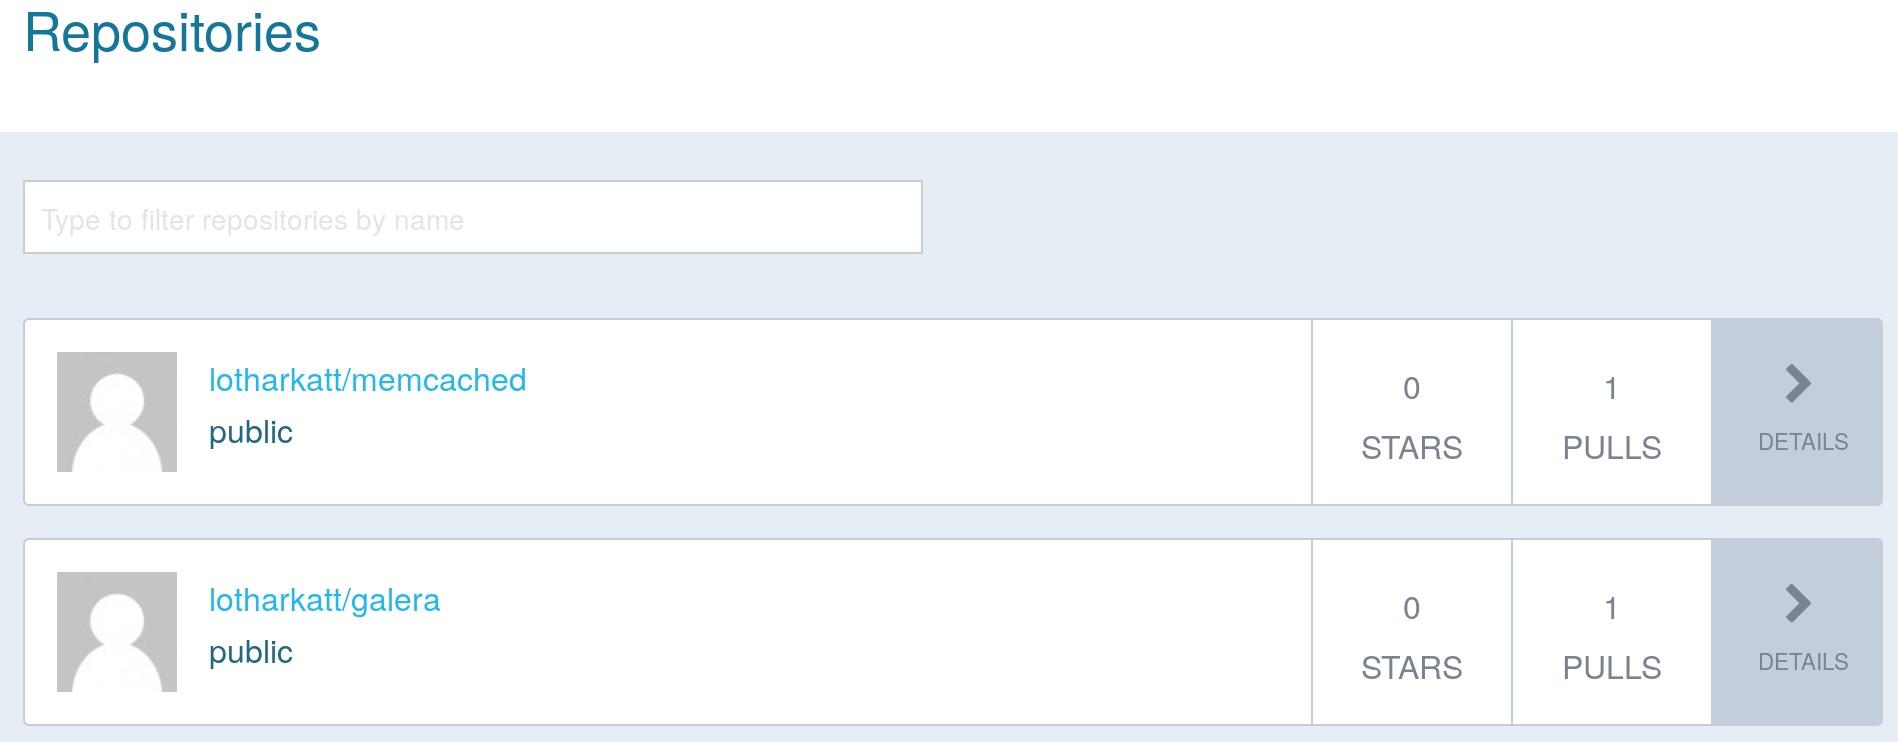
\includegraphics[width=1.0\textwidth]{img/docker_repository}
\par\end{centering}
\caption{Image nahrané na Docker Hub, zdroj: vlastní tvorba \label{fig:docker_repository}}
\end{figure}


\section{Kubernetes}
Pro nasazení kontejnerů do orchestrátoru je nutno napsat konfigurační soubor v formátu yaml. Všechny komponenty Kubernetes se dají nadefinovat pomocí yaml souborů. Pro přehlednost a přístupnost je nutné jednotlivé komponenty a aplikace sdružovat do skupin pomocí namespaců. Pomocí namespacu lze také přidělovat práva jednotlivým uživatelům přistupujícím do Kubernetes clusteru. Je nežádoucí, aby všichni uživatelé měli přístup ke všem aplikacím běžícím na jedné infrastruktuře. Jednotlivé komponenty se zobrazují pomocí přepínače \textit{--namespace <název namespace>}. V této práci tento způsob označování aplikace využit nebyl z důvodu běhu pouze jedné aplikace v Kubernetes clusteru. Celý konfigurační soubor je vysvětlen na ukázce kódu \ref{lst:k8s-1}.

\begin{lstlisting}[caption={Ukázka konfigurace Kubernetes  komponent, část 1},label= {lst:k8s-1}]
---
apiVersion: v1
kind: Namespace
metadata:
  name: web-application
---
\end{lstlisting}

Kubernetes service lze nazvat jako sdružení pravidel, která spojují pody navzájem. Kromě metadat jako je jméno a label, se musí specifikovat porty, přes které budou aplikace dostupné. V případě vzorového kódu \ref{lst:k8s-2} se jedná o port 3306. Pomocí této definice bude port 3306 nastaven kontejnerům uvnitř podu. 

\begin{lstlisting}[caption={Ukázka konfigurace Kubernetes komponent, část 2},label= {lst:k8s-2}]
kind: Service
apiVersion: v1
metadata:
  name: mysql
  labels:
    name: mysql
spec:
  ports:
    - name: mysql
      port: 3306
      protocol: TCP
  selector:
name: mysql
\end{lstlisting}

Deploymentem by se dala označit obecná definice podů. Definice deploymentu určuje, kolik replik a jakou image má obsahovat. Na základně této definice vzniká ReplicaSet (Replication Controller), pomocí kterého se škálují kontejnery. Z ukázky číslo \ref{lst:k8s-3} je vidět základní definici podu. Tato konfigurační část začíná specifikací počtu replik, které budou vytvořené po spuštění yamlu s předpisem pro deployment. Následuje definice pro kontejner,  nastavení image. V základním nastavení je image stahován z veřejného repositáře Docker Hub. Zde je nutné poznamenat, že pokud je vyžadována specifická verze image jako v této práci, je nutné za cestu k image také uvést správnou verzi, jinak kontejner nebude správně spuštěn. Dalším důležitým parametrem je port, který má být pro pod otevřen. V práci se jedná o port 3306, port pro MySql databázi. Poté následuje deklarace enviromentalních proměnných, které jsou vyžadovány pro správný běh databáze. Celá definice je zakončena VolumemMountem. Pomocí této definice je nastaveno, že veškerý obsah adresáře \textit{/var/lib/mysql/} bude přesunut na hostitelský systém do cesty \textit{/home/ubuntu/mysql/}. Pokud by nebyla cesta z kontejneru nadefinovaná, aplikace by po pádu kontejneru přišla o veškerá data. 

\begin{lstlisting}[caption={Ukázka konfigurace Kubernetes komponent, část 3},label= {lst:k8s-3}]
apiVersion: extensions/v1beta1
kind: Deployment
metadata:
  name: mysql
spec:
  replicas: 1
  template:
    metadata:
      labels:
        name: mysql
    spec:
      containers:
      - image: lotharkatt/galera:1.0
        name: mysql
        ports:
        - containerPort: 3306
        env:
        - name: MYSQL_DATABASE
          value: owncloud_db
        - name: MYSQL_USER
          value: admin
        - name: MYSQL_PASSWORD
          value: password 
        volumeMounts:
        - mountPath: /var/lib/mysql/
          name: mysql
      volumes:
        - hostPath:
            path: /home/ubuntu/mysql/
	      name: mysql
\end{lstlisting}

Vytvoření podů pak probíhá zavoláním příkazu \textit{kubectl create -f <cesta k konfiguračnímu yaml souboru>}.  Při spuštění uvedeného Kubernetes konfiguračního souboru pro mysql se spustí dvě komponenty, deployment a service. Součástí deploymentu je také ReplicaSet. Pokud je konfigurace vyplněná správně, při zobrazení listu služeb, bude vyexportován daný port.

Klíčovou vlastnost, kterou je potřeba pro Kubernetes cluster nakonfigurovat, je viditelnost vůči venkovním sítím. Orchestrátor si adresuje pody nezávisle na síťových rozsazích. Pro dostupnost sítí z vnějšího světa lze použít hned několik způsobů přístupu. Nejjednoduší je konfigurace parametru NodePort, pomocí kterého lze vyexportovat port podu přímo na port hostitelského stroje. Tento postup byl použit v této práci. Další možností je nastavení tzv. kube-proxy, jak už název napovídá, jedná se o proxy řešení, přes které lze přistupovat rovněž do venkovní sítě. Pro komunikaci s venkovní sítí také lze použít komponentu ingress, přes kterou je možné přistupovat přímo na servisní porty. 

\subsection{Ukázka škálování}
Kubernetes podporuje horizontální škálování, v následující ukázce kódu \ref{lst:scale-1} je zobrazen výpis jednotlivých podů s jejich stavem. Je vidět, že jednotlivé pody mají alokované IP adresy, které jim přiřadil sám orchestrátor, a fyzická zařízení, na která je umístil scheduler. Automatické adresování kontejnerů je důležité zejména díky škálování, není možné, aby při přidávaní kontejnerů administrátor hlídal adresní rozsahy a adresoval pody ručně. 

\begin{lstlisting}[caption={Ukázka škálování, čast 1},label= {lst:scale-1}]
root@k8s-master:~# kubectl get pods -o wide
NAME                         READY     STATUS    RESTARTS   AGE       IP              NODE
memcached-3034518848-hhpz3   1/1       Running   0          4m        10.233.76.116   k8s-minion-02
mysql-1155545570-1rnms       1/1       Running   0          10m       10.233.76.113   k8s-minion-02
nginx-3571296254-2fkjm       1/1       Running   0          7m        10.233.76.115   k8s-minion-02
owncloud-4254227122-37qfs    1/1       Running   0          23s       10.233.95.54    k8s-minion-01
\end{lstlisting}

Pro zobrazení aktuálního počtu a stavu lze použít deployment list, který zobrazuje aktuální počet jednotlivých podů. Kromě počtu a dostupnosti podů je zde sloupec up-to-date, který při spuštění rolling updatu ukazuje počet aktualizovaných podů. Seznam deploymentů je zobrazen v ukázce kódu \ref{lst:scale-2}

\begin{lstlisting}[caption={Ukázka škálování, čast 2},label= {lst:scale-2}]
root@k8s-master:~# kubectl get deployment 
NAME        DESIRED   CURRENT   UP-TO-DATE   AVAILABLE   AGE
memcached   1         1         1            1           5m
mysql       1         1         1            1           11m
nginx       1         1         1            1           8m
owncloud    1         1         1            1           1m
\end{lstlisting}

Pro vyvolání škálovaní se používá příkaz kubectl, přes který se ovládá celý Kubernetes cluster. Pomocí příkazu {\textit{kubectl scale deployment/owncloud --replicas=5} se vyškálují pody s kontejnery na stanovenou hodnotu, v tomto případě se jedná o pět replik. Proces replikace probíhá následovně: je změněna hodnota replik, ta je odeslána přes API server na ReplicaSet (Replication Controller), ten zavolá scheduler a pošle mu požadovaný počet nových podů, scheduler je pak vytvoří na nodech, kde jsou dostupné zdroje. Škálování podů probíhá paralelně, je spouštěno několik replik najednou. Výsledek vyškálované aplikace je zobrazen na ukázce kódu \ref{lst:scale-3}

\begin{lstlisting}[caption={Ukázka škálování, čast 3},label= {lst:scale-3}]
root@k8s-master:~# kubectl get deployment  
NAME        DESIRED   CURRENT   UP-TO-DATE   AVAILABLE   AGE
memcached   1         1         1            1           7m
mysql       1         1         1            1           13m
nginx       1         1         1            1           9m
owncloud    5         5         5            5           2m
\end{lstlisting}

Pro ověření úspěšného škálování je vhodné zkontrolovat seznam podů, na ukázce kódu \ref{lst:scale-4} lze vidět, že všechny kontejnery byly úspěšně vyškálovány bez jakéhokoliv pádu či restartu. Při srovnání s ukázkou kódu \ref{lst:scale-1} je možno vidět, že původní pod s kontejnery aplikace OwnCloud zůstal nezměněn. 

Pro automatické škálovaní, které v této práci nebude demonstrováno, lze použít jednoduchý předpis buď pro Replication Controller, nebo přímo deployment. Například {\textit{kubectl autoscale deployment owncloud --min=2 --max=5 --cpu-percent=60}, pomocí tohoto příkazu se začne pod automaticky škálovat, jakmile hranice vytížení procesoru kontejneru stoupne nad 60 procent do počtu stanovených replik. Toto je výhodné při velkém vytížení webové aplikace, pokud do ní přistupuje mnoho uživatelů, aplikace se sama automaticky naškáluje. Jakmile zátěž procesoru poklesne, počet podů s kontejnery se opět sníží.

\begin{lstlisting}[caption={Ukázka škálování, čast 4},label= {lst:scale-4}]
root@k8s-master:~# kubectl get pods -o wide
NAME                         READY     STATUS    RESTARTS   AGE       IP              NODE
memcached-3034518848-hhpz3   1/1       Running   0          7m        10.233.76.116   k8s-minion-02
mysql-1155545570-1rnms       1/1       Running   0          13m       10.233.76.113   k8s-minion-02
nginx-3571296254-2fkjm       1/1       Running   0          9m        10.233.76.115   k8s-minion-02
owncloud-4254227122-37qfs    1/1       Running   0          2m        10.233.95.54    k8s-minion-01
owncloud-4254227122-9190b    1/1       Running   0          14s       10.233.76.117   k8s-minion-02
owncloud-4254227122-gmpp8    1/1       Running   0          14s       10.233.95.55    k8s-minion-01
owncloud-4254227122-n77pv    1/1       Running   0          14s       10.233.76.118   k8s-minion-02
owncloud-4254227122-v6dg0    1/1       Running   0          14s       10.233.95.56    k8s-minion-01
\end{lstlisting}

\subsection{Vysoká dostupnost}
Demonstrace vysoké dostupnosti byla provedena na ukázce již naškálované aplikace. Na ukázce kódu \ref{lst:trouble-1} je zobrazen seznam podů před ukázkou vysoké dostupnosti. 

V této ukázce bude z Kubernetes clusteru vyřazen jeden fyzický sever, který slouží jako minion pro běh podů. Výpadek serveru označen jako k8s-minion-01 bude proveden pomocí tvrdého vypnutí serveru přímo přes ILo daného fyzického zařízení.

\begin{lstlisting}[caption={Seznam podů po nainstalovaní Kuberentes},label= {lst:trouble-1}]
root@k8s-master:~# kubectl get pods -o wide
NAME                         READY     STATUS    RESTARTS   AGE       IP              NODE
memcached-3034518848-hhpz3   1/1       Running   0          10m       10.233.76.116   k8s-minion-02
memcached-3034518848-hmvl0   1/1       Running   0          55s       10.233.76.120   k8s-minion-02
memcached-3034518848-vcpgk   1/1       Running   0          55s       10.233.95.59    k8s-minion-01
mysql-1155545570-1rnms       1/1       Running   0          16m       10.233.76.113   k8s-minion-02
mysql-1155545570-647b7       1/1       Running   0          1m        10.233.76.119   k8s-minion-02
mysql-1155545570-7dpg9       1/1       Running   0          1m        10.233.95.58    k8s-minion-01
nginx-3571296254-2fkjm       1/1       Running   0          13m       10.233.76.115   k8s-minion-02
nginx-3571296254-hpnpd       1/1       Running   0          1m        10.233.95.57    k8s-minion-01
owncloud-4254227122-9190b    1/1       Running   0          3m        10.233.76.117   k8s-minion-02
owncloud-4254227122-n77pv    1/1       Running   0          3m        10.233.76.118   k8s-minion-02
\end{lstlisting}

Po vypnutí miniona rozeznal Kubernetes cluster, že minion je nedostupný. V základním nastavení je reakční doba pět minut. Po uplynutí této doby jsou všechny instance z nedostupného nodu přemigrovány na zbylé miniony. Tento fakt je znázorněn na ukázce kódu \ref{lst:trouble-2}. Pody jsou vytvořeny s odlišným jménem a subnetem odpovídajícím rozsahu druhého nodu.

Tento koncept dodává vysokou flexibilitu a dostupnost jednotlivých služeb. Tento proces funguje správně jen díky bezstavovému modelu aplikací, které nejsou v důsledku závislé na hostitelském systému.

\begin{lstlisting}[caption={Seznam podů po nainstalovaní Kuberentes},label= {lst:trouble-2}]
root@k8s-master:~# kubectl get pods -o wide
NAME                         READY     STATUS             RESTARTS   AGE       IP              NODE
memcached-3034518848-69rwq   1/1       Running            0          23m       10.233.76.121   k8s-minion-02
memcached-3034518848-hhpz3   1/1       Running            0          40m       10.233.76.116   k8s-minion-02
memcached-3034518848-hmvl0   1/1       Running            0          30m       10.233.76.120   k8s-minion-02
mysql-1155545570-1rnms       1/1       Running            0          46m       10.233.76.113   k8s-minion-02
mysql-1155545570-647b7       1/1       Running            0          30m       10.233.76.119   k8s-minion-02
mysql-1155545570-vsbd6       1/1       Running            0          23m       10.233.76.122   k8s-minion-02
nginx-3571296254-2fkjm       1/1       Running            0          42m       10.233.76.115   k8s-minion-02
nginx-3571296254-rrm2n       1/1       Running            0          23m       10.233.76.123   k8s-minion-02
owncloud-4254227122-9190b    1/1       Running            0          33m       10.233.76.117   k8s-minion-02
owncloud-4254227122-n77pv    1/1       Running            0          33m       10.233.76.118   k8s-minion-02
\end{lstlisting}
\chapter{Závěry a doporučení}
\section{Závěr}
Kontejnerová virtualizace je zajisté evolucí v moderním světě virtualizace, ve kterém se nyní firmy odklánějí od proprietárních virtualizačních technologií k open source řešením. Kontejnery se svým  přístupem a prací se zdroji mění celkový pohled na virtualizaci, jsou nesrovnatelně rychlejší než klasická virtualizace.

Tato práce si dala za cíl prověřit, zda je možné převést do kontejnerů klasickou aplikaci. V práci byla zmíněna problematika kontejnerové virtualizace. Pomocí vybraných nástrojů byla převedena jednoduchá webová aplikace do kontejnerového prostředí. Na této aplikaci pak bylo demonstrováno několik případů užití orchestrátoru. Z výsledku lze usoudit, že převedení aplikace do kontejnerového prostředí je možné, záleží však na architektuře aplikace a použití dostupných technologií. Využití kontejnerové virtualizace ve standardním podnikovém prostředí bez použití orchestrátoru nedává smysl. 

\section{Budoucnost kontejnerových technologií}
Lze téměř s jistotou tvrdit, že historie se opakovat nebude a kontejnery se už stanou plnohodnotným virtualizačním řešením, které se bude běžně používat v produkčních prostředích. Díky OCi a komunitě okolo alternativních runtime je předpoklad,že  dojde k odklonu od Dockeru, protože jako rkt či cri-o pracuje spolehlivě.

Orchestrátory čeká zajisté podobná cesta jako projekt OpenStack. Velké firmy začínají vydávat své vlastní distribuce, které implementují lepší podporu pro jejich stávající produkty a služby. Kubernetes se už tak dočkal své distribuce od Canonicalu a CoreOS. Firma Redhat si nad Kubernetes postavila celou kontejnerovou platformu OpenShift. Kontejnerová virtualizace se bude zajisté i nadále měnit a rozvíjet.

\addcontentsline{toc}{chapter}{Literatura} 

\begin{thebibliography}{10}

\bibitem{docker_part} 
	\emph{Docker: Customers story}. {[}online] 2017 {[}cit. 2017-5-4]. Dostupné z: \url{https://www.docker.com/customers}

\bibitem{chroot}MATTEO, Riondato. 
  \emph{FreeBSD Handbook Chapter 15 Jails}. freebsd.org. The FreeBSD Project {[}online] 2014 {[}cit. 2017-1-27] Dostupné z: \url{https://www.freebsd.org/doc/en_US.ISO8859-1/books/handbook/jails.html}	
  
\bibitem{solaris_zone} 
	\emph{Solaris Internals wiki:Zones}. {[}online] 2007 {[}cit. 2017-1-27]. Dostupné z: \url{https://solarisinternals.com/wiki/index.php/Zones}	  

\bibitem{gp_38}BOTTOMLEY, James.
	\emph{WHAT IS ALL THE CONTAINER HYPE?}. {[}online] 2014 {[}cit. 2017-1-27]. Dostupné z: \url{https://virtuozzo.com/wp-content/uploads/2016/03/Virtuozzo_Container-Hype_WP_Ltr_2015_March2016.pdf}
    
\bibitem{windows_container}
	\emph{Windows Containers}. {[}online] 2016 {[}cit. 2017-2-4]. Dostupné z: \url{https://docs.microsoft.com/en-us/virtualization/windowscontainers/about/}
       
\bibitem{dotcloud_docker}GLOUB, Ben.
	\emph{DotCloud, Inc. is Becoming Docker, Inc}. {[}online] 2013 {[}cit. 2017-2-4]. Dostupné z: \url{https://blog.docker.com/2013/10/dotcloud-is-becoming-docker-inc/}

\bibitem{docker_mil}KONRAD, Alex.
	\emph{Forbes: Open-Source Darling Docker Cracks The Billion-Dollar Club With \$95 Million Raise}. {[}online] 2015 {[}cit. 2017-2-15]. Dostupné z: \url{https://www.forbes.com/sites/alexkonrad/2015/04/14/docker-raises-95-million-at-billion-valuation/}

\bibitem{cluster_vyzkum}FERRANTI, Alex.
	\emph{Survey: 96\% increase in container production usage over past year}. {[}online] 2016 {[}cit. 2017-2-17]. Dostupné z: \url{https://blog.docker.com/2013/10/dotcloud-is-becoming-docker-inc/}

\bibitem{oci_born}Open Container Initiative
	\emph{Industry Leaders Unite to Create Project for Open Container Standards}. {[}online] 2015 {[}cit. 2017-2-17]. Dostupné z: \url{https://www.opencontainers.org/announcement/2015/06/20/industry-leaders-unite-to-create-project-for-open-container-standards}

\bibitem{docker_1_12}Docker Core Engineering.
	\emph{Docker 1.12: Now with Built-in Orchestration!}. {[}online] 2016 {[}cit. 2017-3-20]. Dostupné z: \url{https://blog.docker.com/2016/06/docker-1-12-built-in-orchestration/}	


\bibitem{Docker_OD} HOLLA, Shrikrishna. 
  \emph{Orchestrating Docker}. Packt Publishing Limited, 2015, 154 s. ISBN 978-1-783-98478-7

%\bibitem{swarm_arch} Docker Documentation 
%	\emph{Docker Documentation:Swarm mode overview}. {[}online] 2016 {[}cit. 2017-XX-XX]. Dostupné z: \url{https://docs.docker.com/engine/swarm/}

\bibitem{docker_lib} HYKES, Solomon.
	\emph{Docker 0.9: introducing execution drivers and libcontainer}. {[}online]. 2014 {[}cit. 2017-3-25]. Dostupné z: \url{https://blog.docker.com/2014/03/docker-0-9-introducing-execution-drivers-and-libcontainer/}

\bibitem{coreos_00} PHILIPS, Brandon.
	\emph{rkt: initial commit}. {[}online]. 2014 {[}cit. 2017-3-27]. Dostupné z: \url{https://github.com/rkt/rkt/releases/tag/v0.0.0}

\bibitem{kube_incubator}Kubernetes komunita
	\emph{Github: Kubernetes-incubator}. {[}online]. 2016 {[}cit. 2017-3-28]. Dostupné z: \url{https://github.com/kubernetes-incubator}

\bibitem{cri_o_inc}Kubernetes komunita
	\emph{Github: Cri-o}. {[}online]. 2016 {[}cit. 2017-3-28]. Dostupné z: \url{https://github.com/kubernetes-incubator/cri-o}

\bibitem{cri_o}
	\emph{Github: Cri-o: Releases}. {[}online] 2017 {[}cit. 2017-3-28]. Dostupné z: \url{https://github.com/kubernetes-incubator/cri-o/releases/tag/v0.1}


\bibitem{beda_prez}BEDA, Joe.
	\emph{Containers At Scale}. {[}online] 2017 {[}cit. 2017-3-28]. Dostupné z: \url{https://speakerdeck.com/jbeda/containers-at-scale}	

\bibitem{docker_1_0}BARBIER, Julien.
	\emph{It’s Here: Docker 1.0}. {[}online]. 2014 {[}cit. 2017-3-28]. Dostupné z: \url{https://blog.docker.com/2014/06/its-here-docker-1-0/}

\bibitem{K8S_micro} VOHRA, Deepak. 
  \emph{Kubernetes Microservices with Docker}. Berkley, United States, 2016, 432 s. ISBN 978-1-484-21906-5

\bibitem{lb_ha}HEIDI, Erika.
	\emph{What Makes a System Highly Available?}. {[}online]. 2016 {[}cit. 2017-4-4]. Dostupné z: \url{https://www.digitalocean.com/community/tutorials/what-is-high-availability}

\bibitem{Docker_doc_layers} Docker Documentation
	\emph{Docker Documentation: Understand images, containers, and storage drivers}. {[}online] 2016 {[}cit. 2017-4-4]. Dostupné z: \url{https://docs.docker.com/engine/userguide/storagedriver/imagesandcontainers/}

\bibitem{fleet_systemd}Systemd doc tým
	\emph{systemd System and Service Manager}. {[}online] 2017 {[}cit. 2017-4-7]. Dostupné z: \url{https://www.freedesktop.org/wiki/Software/systemd/}	

\bibitem{fleet_lim}CoreOS tým
	\emph{CoreOS: fleet and scaling}. {[}online] 2016 {[}cit. 2017-4-8]. Dostupné z: \url{https://github.com/coreos/fleet/blob/master/Documentation/fleet-scaling.md}	

\bibitem{fleet_end}WOOD, Josh.
	\emph{Container orchestration: Moving from fleet to Kubernetes}. {[}online] 2017 {[}cit. 2017-4-8]. Dostupné z: \url{https://coreos.com/blog/migrating-from-fleet-to-kubernetes.html}	
  
\bibitem{swarm_compose} Docker Documentation 
	\emph{Docker Documentation:Use Compose with Swarm}. {[}online] 2016 {[}cit. 2017-4-8]. Dostupné z: \url{https://docs.docker.com/compose/swarm/}    

\bibitem{mesos} HINDMAN, Benjamin, KONWINSKI Andy, ZAHARIA, Matei, GHODSI Alii, JOSEPH D., Anthony, KATZ, Randy, SHENKER, Scoot, Stoica Ion. 
	\emph{Mesos: A Platform for Fine-Grained Resource Sharing in the Data Center}. {[}online] 2010 {[}cit. 2017-4-9]. Dostupné z: \url{http://mesos.berkeley.edu/mesos_tech_report.pdf}   

\bibitem{k8s_kuba} RENSIN, David K. 
  \emph{Kubernetes Scheduling the Future at Cloud Scale}. O'Reilly, United States, 2015, 38 s. ISBN 978-1-491-93599-6

\bibitem{Docker_learning} RAJ,  Pethuru, SINGH, Vinod, CHELLADHURAI, Jeeva S. 
  \emph{Learning Docker}. Packt Publishing Limited, 2015, 240 s. ISBN 978-1-784-39793-7

\bibitem{Docker_vs_rkt} rkt Documentationn
	\emph{rkt Documentation: rkt vs other projects}. {[}online] 2016 {[}cit. 2017-4-12]. Dostupné z: \url{https://coreos.com/rkt/docs/latest/rkt-vs-other-projects.html}

\bibitem{ngnix} W3techs tým
    \emph{W3techs: Usage of web servers for websites}. {[}online] 2015 {[}cit. 2017-4-17]. Dostupné z: \url{https://w3techs.com/technologies/overview/web_server/all}

\bibitem{ms_ms} rkt Documentationn
	\emph{Microsoft Azure - Azure Service Fabric and the Microservices Architecture}. {[}online] 2016 {[}cit. 2017-4-19]. Dostupné z: \url{https://msdn.microsoft.com/en-us/magazine/mt595752.aspx}

\bibitem{ubuntu_alpine} gliderlabs/docker-alpine
	\emph{Docker Alpine Linux}. {[}online] 2016 {[}cit. 2017-4-19]. Dostupné z: \url{https://github.com/gliderlabs/docker-alpine#usage}

\bibitem{swarm_arch} Docker Documentation 
	\emph{Docker Documentation:Swarm mode overview}. {[}online] 2016 {[}cit. 2017-3-26]. Dostupné z: \url{https://docs.docker.com/engine/swarm/}
	
\end{thebibliography}


\cleardoublepage{}

%\chapter{Přílohy}
\pagenumbering{arabic}
\setcounter{page}{1}




4ka predsivt

jak to bezi virtualky, zdroje atd...

statefull s
stateless
--vysvetli rozdelit  do dvou odstavcu

popis aplikace obrzazek

kontjenrova technologie
refrencovat se na horu


5 migrace
architektura nahoru


zaver 
mas smysl nema smysl
\section{A. Manuál k migrované aplikaci}







\appendix
\pagenumbering{Roman}

\chapter{Cizí výrazy}
\begin{itemize}
\item cgroups, namespaces - Linuxové zdroje zabudované v kernelu, pomocí který se izolují kontejnerové technologie od hostitelského systému.
\item VM(Virtual Machine) - Virtuální stroj - Jedná se o produkt virtualizace, jedná se o software, který emuluje hardware a dokáže tak spustit operační systém, který má obdobné vlastnosti jako operační systém nainstalovaný na hardwaru.
\item Hardware - Fyzicky existujicí technické vybavení počítače.
\item Open source - Otevřený kód, progamy označovaný open source má volně přístupné zdrojové kódy většinou se tyto kódy nachází na serveru GitHub.
\item Linoxový daemon - Program, který je spuštěn dlouhodobě, není v přímém kontakt s uživatelem
\item Hypervisor - Hostitelský operační systém, který řídí přístup k virtualizovaným systémům
\item Runtime - Knihovny potřebné k spustění aplikace
\item Microslužby - Je tip architektury, která staví svůj koncept na rozdělení služeb nezávislých celků. 
\item Git - je SCM nástroj na správu verzi Softwarů, autorem je Linus Torvalds (autor Linuxové kernelu) 
\item Linuxový kernel - Monolithické jádro, které ovládá a spravuje hardwarové zdroje, jedná se zároveň na největší open source projekt. 
\item GitHub - Největší veřejný repozitář pro ukládání kódu v systému gitu.
\item Single point of failure - Je část aplikace, která při své nedostupnosti může způsobit výpadky celé aplikace.
\item Cluster - Jedná se o skupinu propojených služeb/počítačů, které navzájem spolupracují
\item init - Proces, který je spuštěn v unixových systémech jako první.
\item Scheduler - Technologie, které slouží k plánování a spouštěním procesů na jednou. 
\end{itemize}

\listoffigures
\listoftables
\lstlistoflistings

%zadani
%\includepdf[pages={1},scale=0.8]{zadani2}
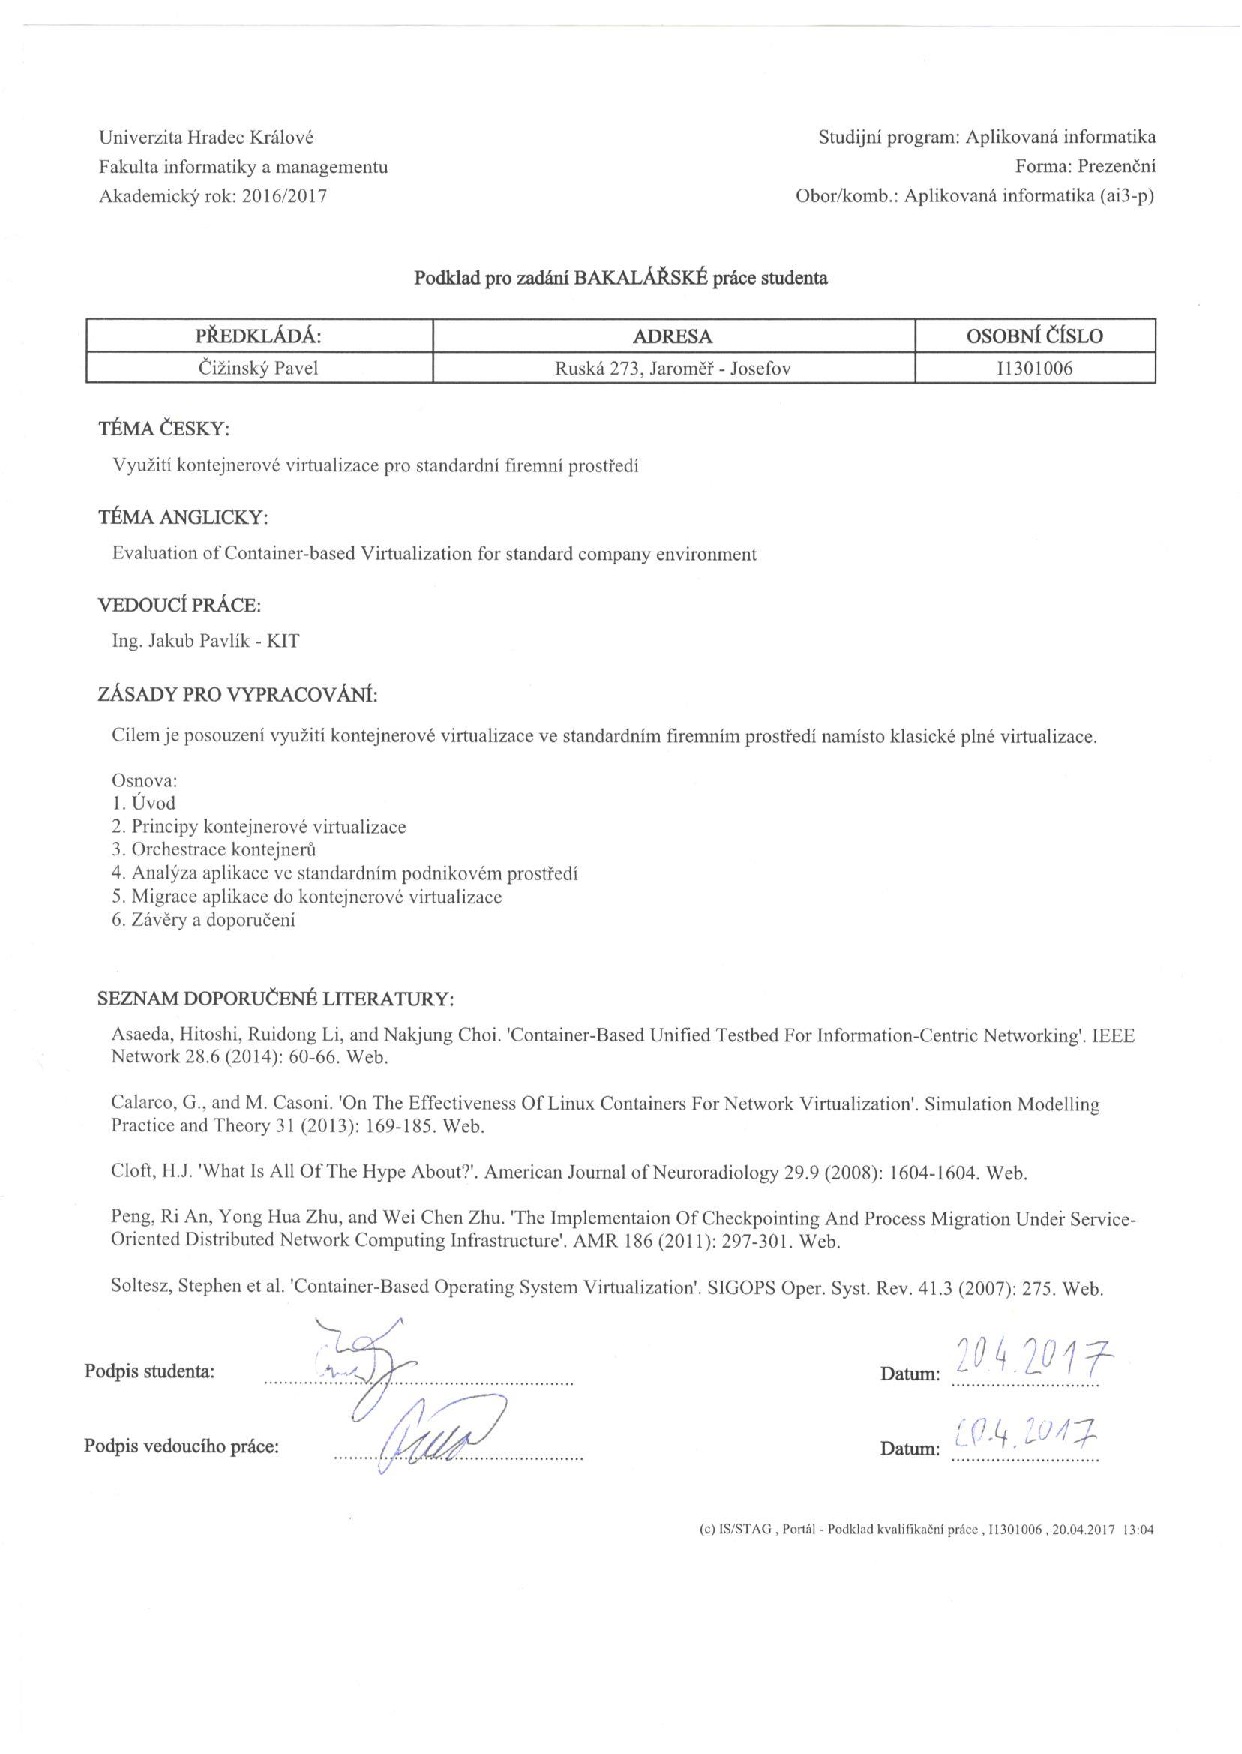
\includepdf[pages={1}]{zadani.pdf}

\clearpage{}
\end{document}
